\documentclass{sprawozdanie-agh}
\title{AiMO - strefa płatnego parkowania}
\usepackage{lscape}
\usepackage[final]{pdfpages}
\usepackage[utf8]{inputenc}
\usepackage{listings}
\usepackage{indentfirst}
\usepackage{geometry}
\usepackage{sectsty}
\sectionfont{\fontsize{18}{22}\selectfont}
\usepackage{array}
\usepackage{lscape}
\usepackage[final]{pdfpages}
\newcolumntype{L}[1]{>{\raggedright\let\newline\\\arraybackslash\hspace{0pt}}m{#1}}
\geometry{
 a4paper,
 total={170mm,257mm},
 left=20mm,
 right=20mm,
 top=35mm,
}

\makeatletter

\begin{document}

\przedmiot{Analiza i Modelowanie Oprogramowania}
\tytul{Projekt aplikacji do zarządzania parkingiem}
\podtytul{...}
\kierunek{Informatyka}
\autor{Patryk Gałczyński}
\data{Kraków, 27 stycznia 2017}

\stronatytulowa{}

\newpage
\section{Analiza wymagań systemu:}
\Large
Projekt zakłada modelowanie systemu zarządzania parkingiem. \\

Parking obsługuje klientów indywidualnych oraz firmy. Rezerwacji miejsca będzie można dokonywać telefonicznie, przez stronę WWW oraz na miejscu w automatycznej kasie. Klienci będą mieli możliwość płatności gotówką, kartą (tylko na~miejscu) lub online za pomocą systemu płatności elektronicznej (przelew). \\

Klienci indywidualni płacą za miejsce z góry za określony czas. Klientom biznesowym cyklicznie wystawiana jest zbiorcza faktura za wszystkie rezerwacje z~danego miesiąca. \\

Automatyczna kasa sprzedaje rezerwację na miejscu, udziela informacji o~ilości dostępnych miejsc, umożliwia odebranie rezerwacji złożonej online, przydziela konkretne miejsce. \\

Parkingowy okresowo sprawdza ważność rezerwacji miejsca danego pojazdu. W~przypadku przekroczenia czasu dostępnego na bilecie informuje klienta o zaistniałej sytuacji (telefon/email). W~przypadku braku wyjaśnienia ze strony klienta, parkingowy zamawia pomoc drogową do odholowania pojazdu. \\

Pomoc drogowa eksmituje pojazdy wskazane przez parkingowego jako nie opłacone. \\

System przechowywania danych pozwala na zapis oraz odczyt danych systemu.
\newpage
\section{Aktorzy}
\subsection{Klient}

Podmiot zewnętrzny (osoba lub przedsiębiorstwo), rezerwuje miejsce osobiście lub przez telefon/online, może płacić gotówką, kartą (na miejscu) lub online (karta, przelew), żąda dowodu zakupu (paragon/faktura), składa reklamacje,  opłaca ewentualne kary.

\subsection{Kasa automatyczna}

Element systemu sprzedający rezerwacje na miejsce, udziela informacji o miejscach, przydziela miejsce parkingowe, przyjmuje płatności, wystawia dowód zakupu (paragon).

\subsection{Dział obsługi klienta}

Użytkownik systemu przyjmujący reklamacje, wystawiający faktury dla klientów biznesownych,  przyjmujący opłaty karne (mandaty), generujący raport za~cały miesiąc dla biznesu.

\subsection{Parkingowy}

Użytkownik systemu, sprawdza ważność rezerwacji miejsca, informuje klienta o stanie rezerwacji, zamawia pomoc drogową, generuje raporty podsumowujące dany miesiąc (ilość mandatów, ilość eksmisji), wystawia mandaty za przekroczenie czasu.

\subsection{System przechowywania danych}

Element systemu odpowiadający za zapis oraz odczyt danych o wolnych/zajętych miejscach, klientach oraz wystawionych mandatach.

\subsection{Pomoc drogowa}

Użytkownik systemu, eksmituje niepożądane pojazdy.



\newpage
\section{diagram przypadkow uzycia}
\begin{figure}
\vspace{-2cm}
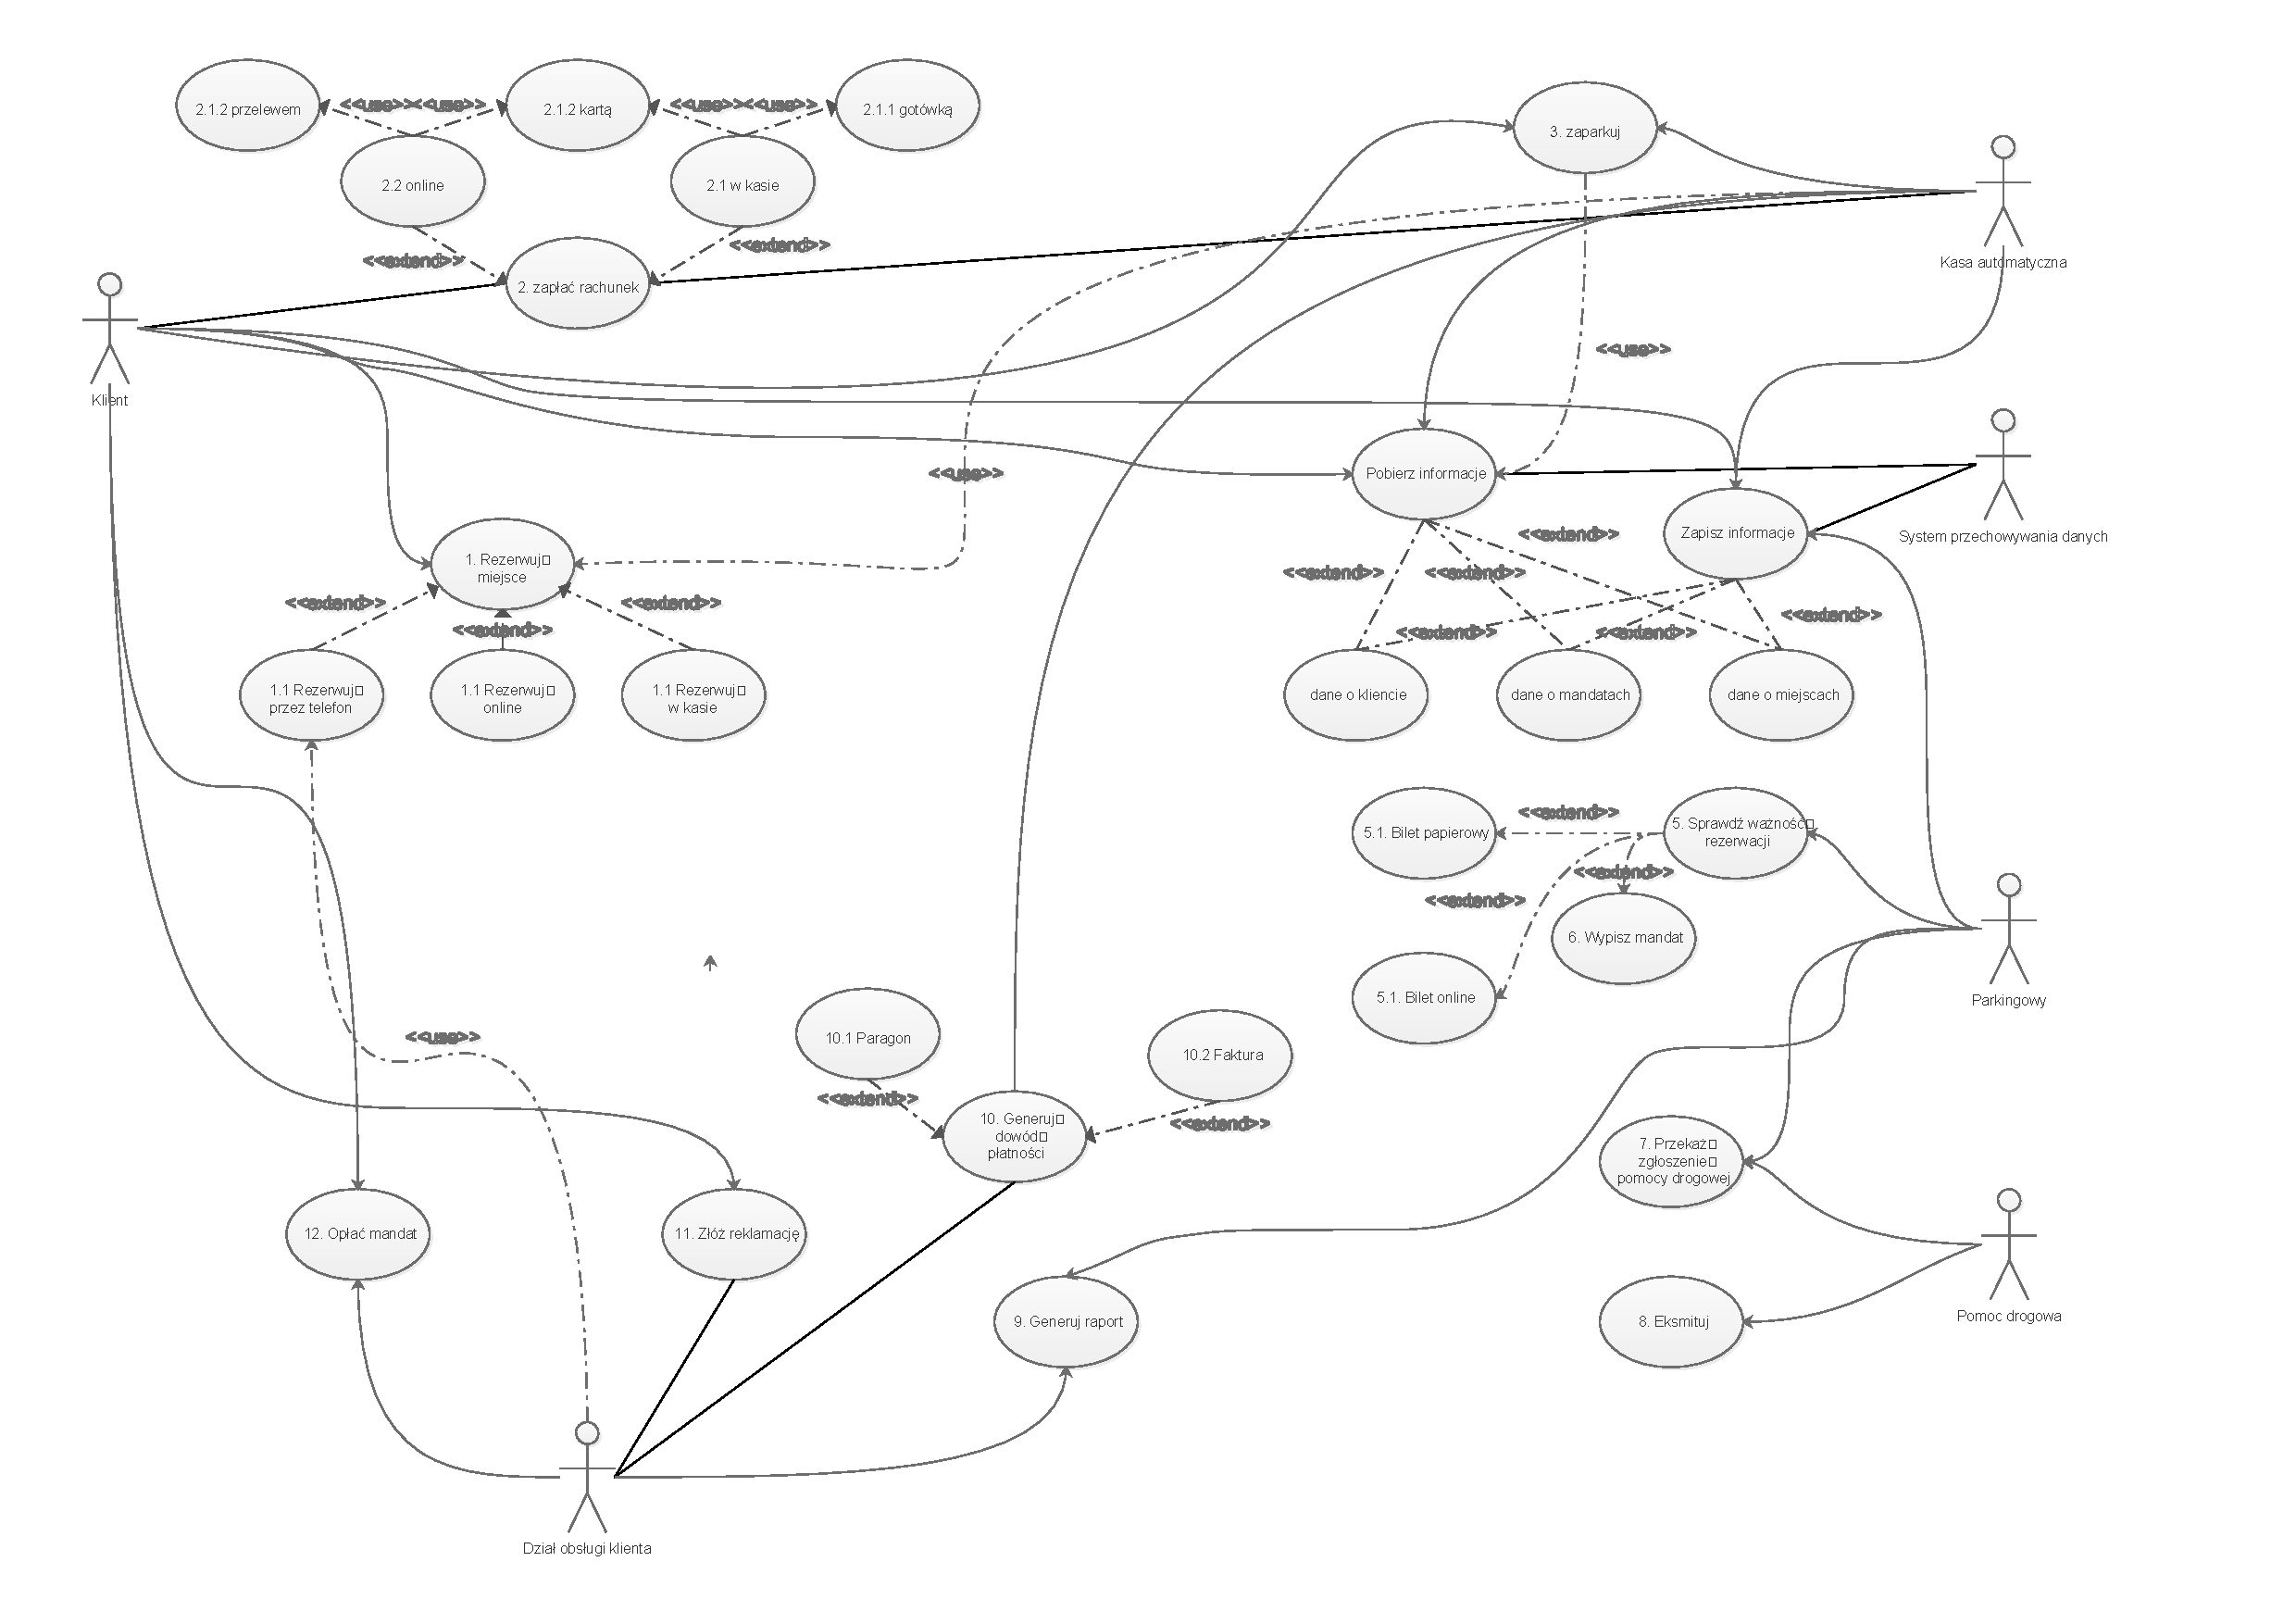
\includepdf[trim=0cm 0 0 -1cm]{uzycia/usecase}
\end{figure}
%\begin{landscape}
%\includegraphics[scale=0.65]{use-case}
%\end{landscape}

\newpage
\section{scenariusze przypadków użycia}
\begin{center}
\begin{tabular}{|L{3cm}  L{13cm}|}
\hline
Nazwa: & 1.1 Rezerwacja miejsca online - płatność kartą \\ \hline
Aktorzy: & Klient,  Automatyczna kasa \\ \hline
Podstawowy ciąg zdarzeń: & 1. Klient wchodzi na stronę www \\
 & 2. Klient wybiera datę i ilość godzin rezerwacji \\
 & 3. Klient zgłasza chęć zrobienia rezerwacji \\
 & 4. Automatyczna kasa rejestruje rezerwację \\
 & 5. Automatyczna kasa wysyła potwierdzenie zrobienia rezerwacji \\
 & 6. Klient dokonuje płatności kartą \\ \hline
Alternatywny ciąg zdarzeń:  & \# Klient rezygnuje z rezerwacji \\
 & \# Klient zmienia datę i ilość godzin w rezerwacji \\
 & \# Automatyczna kasa zwraca informację o braku miejsca w danym terminie\\ 
 \\ \hline
\end{tabular}

\vspace{1cm}

\begin{tabular}{|L{3cm}  L{13cm}|}
\hline
Nazwa: & 1.3 Rezerwacja miejsca online - płatność przelew \\ \hline
Aktorzy: & Klient,  Automatyczna kasa \\ \hline
Podstawowy ciąg zdarzeń: & 1. Klient wchodzi na stronę www \\
 & 2. Klient wybiera datę i ilość godzin rezerwacji \\
 & 3. Klient zgłasza chęć zrobienia rezerwacji \\
 & 4. Automatyczna kasa rejestruje rezerwację \\
 & 5. Automatyczna kasa wysyła potwierdzenie zrobienia rezerwacji \\
 & 6. Klient dokonuje płatności przelewem \\ \hline
Alternatywny ciąg zdarzeń:  & \# klient rezygnuje z rezerwacji \\
 & \# klient zmienia datę i ilość godzin w rezerwacji \\ 
 & \# Automatyczna kasa zwraca informację o braku miejsca w danym terminie\\ \hline
\end{tabular}

\vspace{1cm}

\begin{tabular}{|L{3cm}  L{13cm}|}
\hline
Nazwa: & 1.4 Rezerwacja na miejscu - płatność kartą \\ \hline
Aktorzy: & Klient,  Automatyczna kasa \\ \hline
Podstawowy ciąg zdarzeń: & 1. Klient przyjeżdza na parking \\
 & 2. Klient wybiera długość postoju \\
 & 4. Automatyczna kasa rejestruje rezerwację \\
 & 5. Automatyczna kasa pokazuje informację o dostępności miejsc \\
 & 6. Klient dokonuje płatności kartą \\
 & 7. Automatyczna kasa generuje potwierdzenie zapłaty - paragon \\ \hline
Alternatywny ciąg zdarzeń:  & \# klient rezygnuje z rezerwacji \\
 & \# klient zmienia ilość godzin w rezerwacji \\ 
 & \# Automatyczna kasa zwraca informację o aktualnym braku miejsca\\ 
 & \# Automatyczna kasa zwraca informację o braku środków na koncie \\ \hline
\end{tabular}

\vspace{1cm}

\begin{tabular}{|L{3cm}  L{13cm}|}
\hline
Nazwa: & 1.5 Rezerwacja na miejscu - płatność gotówką \\ \hline
Aktorzy: & Klient,  Automatyczna kasa \\ \hline
Podstawowy ciąg zdarzeń: & 1. Klient przyjeżdza na parking \\
 & 2. Klient wybiera długość postoju \\
 & 4. Automatyczna kasa rejestruje rezerwację \\
 & 5. Automatyczna kasa pokazuje informację o dostępności miejsc \\
 & 6. Klient dokonuje płatności gotówką \\
 & 7. Automatyczna kasa generuje potwierdzenie zapłaty - paragon \\ \hline
Alternatywny ciąg zdarzeń:  & \# klient rezygnuje z rezerwacji \\
 & \# klient zmienia ilość godzin w rezerwacji \\ 
 & \# Automatyczna kasa zwraca informację o aktualnym braku miejsca\\ \hline
\end{tabular}

\vspace{1cm}

\begin{tabular}{|L{3cm}  L{13cm}|}
\hline
Nazwa: & 3 Zaparkowanie pojazdu \\ \hline
Aktorzy: & Klient,  Automatyczna kasa \\ \hline
Podstawowy ciąg zdarzeń: & 1. Klient zgłasza chęć odebrania rezerwacji miejsca w kasie automatycznej\\
 & 2. Kasa automatyczna przydziela klientowi wolne miejsce\\
 & 3. Klient parkuje pojazd w określonym miejscu\\ \hline
Alternatywny ciąg zdarzeń:  & \# klient rezygnuje z rezerwacji \\
 & \# Automatyczna kasa zwraca informację o braku miejsca\\ \hline
\end{tabular}

\vspace{1cm}

\begin{tabular}{|L{3cm}  L{13cm}|}
\hline
Nazwa: & 4. Sprawdzenie dostępności miejsca przez WWW \\ \hline
Aktorzy: & Klient,  Automatyczna kasa \\ \hline
Podstawowy ciąg zdarzeń: & 1. Klient wchodzi na stronę WWW \\
 & 2. Klient wybiera opcję sprawdzenia miejsca \\
 & 3. Automatyczna kasa sprawdza dostępne miejsca \\
 & 4. Automatyczna kasa zwraca informację do WWW \\ \hline
\end{tabular}

\vspace{1cm}

\begin{tabular}{|L{3cm}  L{13cm}|}
\hline
Nazwa: & 5.1 Sprawdzenie ważności biletu - bilet papierowy - bilet nie ważny krótką chwilę\\ \hline
Aktorzy: & Parkingowy, Klient \\ \hline
Podstawowy ciąg zdarzeń: & 1. Parkingowy sprawdza stan biletu papierowego w samochodzie klienta \\
 & 2  Parkingowy dzwoni do klienta aby uzyskać od niego informacje\\
 & 3.1 Parkingowy czeka na klienta \\
 & 3.2 Parkingowy wystawia mandat \\
 & 3.2. Parkingowy zapisuje mandat w systemie \\
 \hline
\end{tabular}

\vspace{1cm}

\begin{tabular}{|L{3cm}  L{13cm}|}
\hline
Nazwa: & 5.2 Sprawdzenie ważności biletu - bilet online - bilet nie ważny krótką chwilę\\ \hline
Aktorzy: & Parkingowy, Klient \\ \hline
Podstawowy ciąg zdarzeń: & 1. Parkingowy sprawdza stan biletu online w systemie poprzez wpisanie numeru rejestracyjnego klienta \\
 & 2  Parkingowy dzwoni do klienta aby uzyskać od niego informacje\\
 & 3.1 Parkingowy czeka na klienta \\
 & 3.2 Parkingowy wystawia mandat \\
 & 3.2 Parkingowy zapisuje mandat w systemie \\
 \hline
\end{tabular}

\vspace{1cm}

\begin{tabular}{|L{3cm}  L{13cm}|}
\hline
Nazwa: & 7 Eksmisja pojazdu\\ \hline
Aktorzy: & Parkingowy, Pomoc drogowa \\ \hline
Podstawowy ciąg zdarzeń: & 1. Parkingowy stwiedza nie opłaconą rezerwację oraz brak kontaktu z klientem\\
 & 2 Parkingowy dzwoni po pomoc drogową\\
 & 3 Pomoc drogowa odholowuje pojazd klienta \\
 \hline
\end{tabular}

\vspace{1cm}

\begin{tabular}{|L{3cm}  L{13cm}|}
\hline
Nazwa: & 9.1 Generowanie raportu miesięcznego przychodów\\ \hline
Aktorzy: & Dział obsługi klienta \\ \hline
Podstawowy ciąg zdarzeń: & 1.  Dział obsługi klienta zostaje powiadomiony o konieczności wygenerowania raportu za dany miesiąc\\
 & 2. Dział obsługi klienta generuje raport z systemu\\
 & 3. Dział obsługi klienta analizuje raport i dopisuje komentarz \\
 \hline
\end{tabular}

\vspace{1cm}

\begin{tabular}{|L{3cm}  L{13cm}|}
\hline
Nazwa: & 9.2 Generowanie raportu miesięcznych wystawionych mandatów\\ \hline
Aktorzy: & Parkingowy \\ \hline
Podstawowy ciąg zdarzeń: & 1. Parkingowy zleca wygenerowanie raportu wystawionych mandatów do systemu\\
 & 2. Parkingowy sprawdza poprawność ze stanem faktycznym za dany miesiąc\\
 & 3. Parkingowy dodaje komentarz, podpisuje dokument\\
 \hline
\end{tabular}


\vspace{1cm}

\begin{tabular}{|L{3cm}  L{13cm}|}
\hline
Nazwa: & 10. Wystawianie faktur za dany okres klientom biznesowym \\ \hline
Aktorzy: & Klient,  Dział obsługi klienta \\ \hline
Podstawowy ciąg zdarzeń: & 1. Klient żąda wydania faktury za dany okres \\
 & 2. Dział obsługi klienta generuje fakturę \\
 & 4. Dział obsługi klienta wysyła fakturę do klienta online \\ \hline
Alternatywny ciąg zdarzeń:  & \# klient rezygnuje z rezerwacji \\
 & \# akcja zapoczątkowana zdarzeniem z timera (generowanie faktury raz w miesiącu) \\ \hline
\end{tabular}

\vspace{1cm}

\begin{tabular}{|L{3cm}  L{13cm}|}
\hline
Nazwa: & 11.1 Klient składa reklamację online\\ \hline
Aktorzy: & Klient, Dział obsługi klienta \\ \hline
Podstawowy ciąg zdarzeń: & 1. Klient wchodzi na stronę WWW \\
 & 2. Klient wypełnia i wysyła formularz reklamacyjny \\
 & 3. Dział obsługi klienta rozpatruje reklamację w ciągu 30 dni robocznych\\
 & 4. Dział obsługi klienta wysyła zawiadomienie o rozpatrzeniu reklamacji \\
 \hline
Alternatywny ciąg zdarzeń:  & \# klient rezygnuje ze składania reklamacji \\
 & \# Dział obsługi klienta powiadamia klienta o zwiększeniu czasu rozpatrywania reklamacji \\ 
 \hline
\end{tabular}

\vspace{1cm}

\begin{tabular}{|L{3cm}  L{13cm}|}
\hline
Nazwa: & 11.2 Klient składa reklamację na miejscu\\ \hline
Aktorzy: & Klient, Dział obsługi klienta \\ \hline
Podstawowy ciąg zdarzeń: & 1. Klient przychodzi do działu obsługi klienta \\
 & 2. Klient wypełnia formularz reklamacyjny \\
 & 3. Pracownik działu obsługi klienta rozpatruje reklamację na miejscu \\
 & 4. Pracownik działu obsługi klienta informuje klienta o rozpatrzeniu reklamacji \\
 \hline
Alternatywny ciąg zdarzeń:  & \# Dział obsługi klienta powiadamia klienta o zwiększeniu czasu rozpatrywania reklamacji \\ 
 \hline
\end{tabular}

\vspace{1cm}

\begin{tabular}{|L{3cm}  L{13cm}|}
\hline
Nazwa: & 12.1 Opłacenie mandatu - paragon\\ \hline
Aktorzy: & Klient,  Dział obsługi klienta \\ \hline
Podstawowy ciąg zdarzeń: & 1. Klient przychodzi do działu obsługi klienta \\
 & 2. Klient przekazuje mandat pracownikowi działu obsługi klienta \\
 & 3. Pracownik działu obsługi klienta przyjmuje płatność od klienta \\
 & 4. Pracownik działu obsługi klienta wystawia paragon opłacenia mandatu \\
 & 5. Pracownik działu obsługi klienta wydaje kartę wyjazdową klientowi \\
 \hline
Alternatywny ciąg zdarzeń:  & \# Klient odmawia przyjęcia mandatu, składa reklamację \\ 
 \hline
\end{tabular}

\vspace{1cm}

\begin{tabular}{|L{3cm}  L{13cm}|}
\hline
Nazwa: & 12.2 Opłacenie mandatu - faktura\\ \hline
Aktorzy: & Klient,  Dział obsługi klienta \\ \hline
Podstawowy ciąg zdarzeń: & 1. Klient przychodzi do działu obsługi klienta \\
 & 2. Klient przekazuje mandat pracownikowi działu obsługi klienta \\
 & 3. Pracownik działu obsługi klienta przyjmuje płatność od klienta \\
 & 4. Pracownik działu obsługi klienta wystawia fakturę opłacenia mandatu \\
 & 5. Pracownik działu obsługi klienta wydaje kartę wyjazdową klientowi \\
 \hline
Alternatywny ciąg zdarzeń:  & \# Klient odmawia przyjęcia mandatu, składa reklamację \\ 
 \hline
\end{tabular}
\end{center}
\newpage
\section{Diagramy sekwencji}
\subsection{Rezerwacja online}
\subsection{Rezerwacja na miejscu}
\subsection{Zaparkowanie pojazdu}
\subsection{Sprawdzenie dostępności przez WWW}
\subsection{Wystawienie mandatu i odholowanie pojazdu}
\subsection{Raport mandatowy oraz finansowy}
\subsection{Wystawianie faktur}
\subsection{Reklamacje}
\subsection{Opłacenie mandatu}
\begin{center}
\newpage
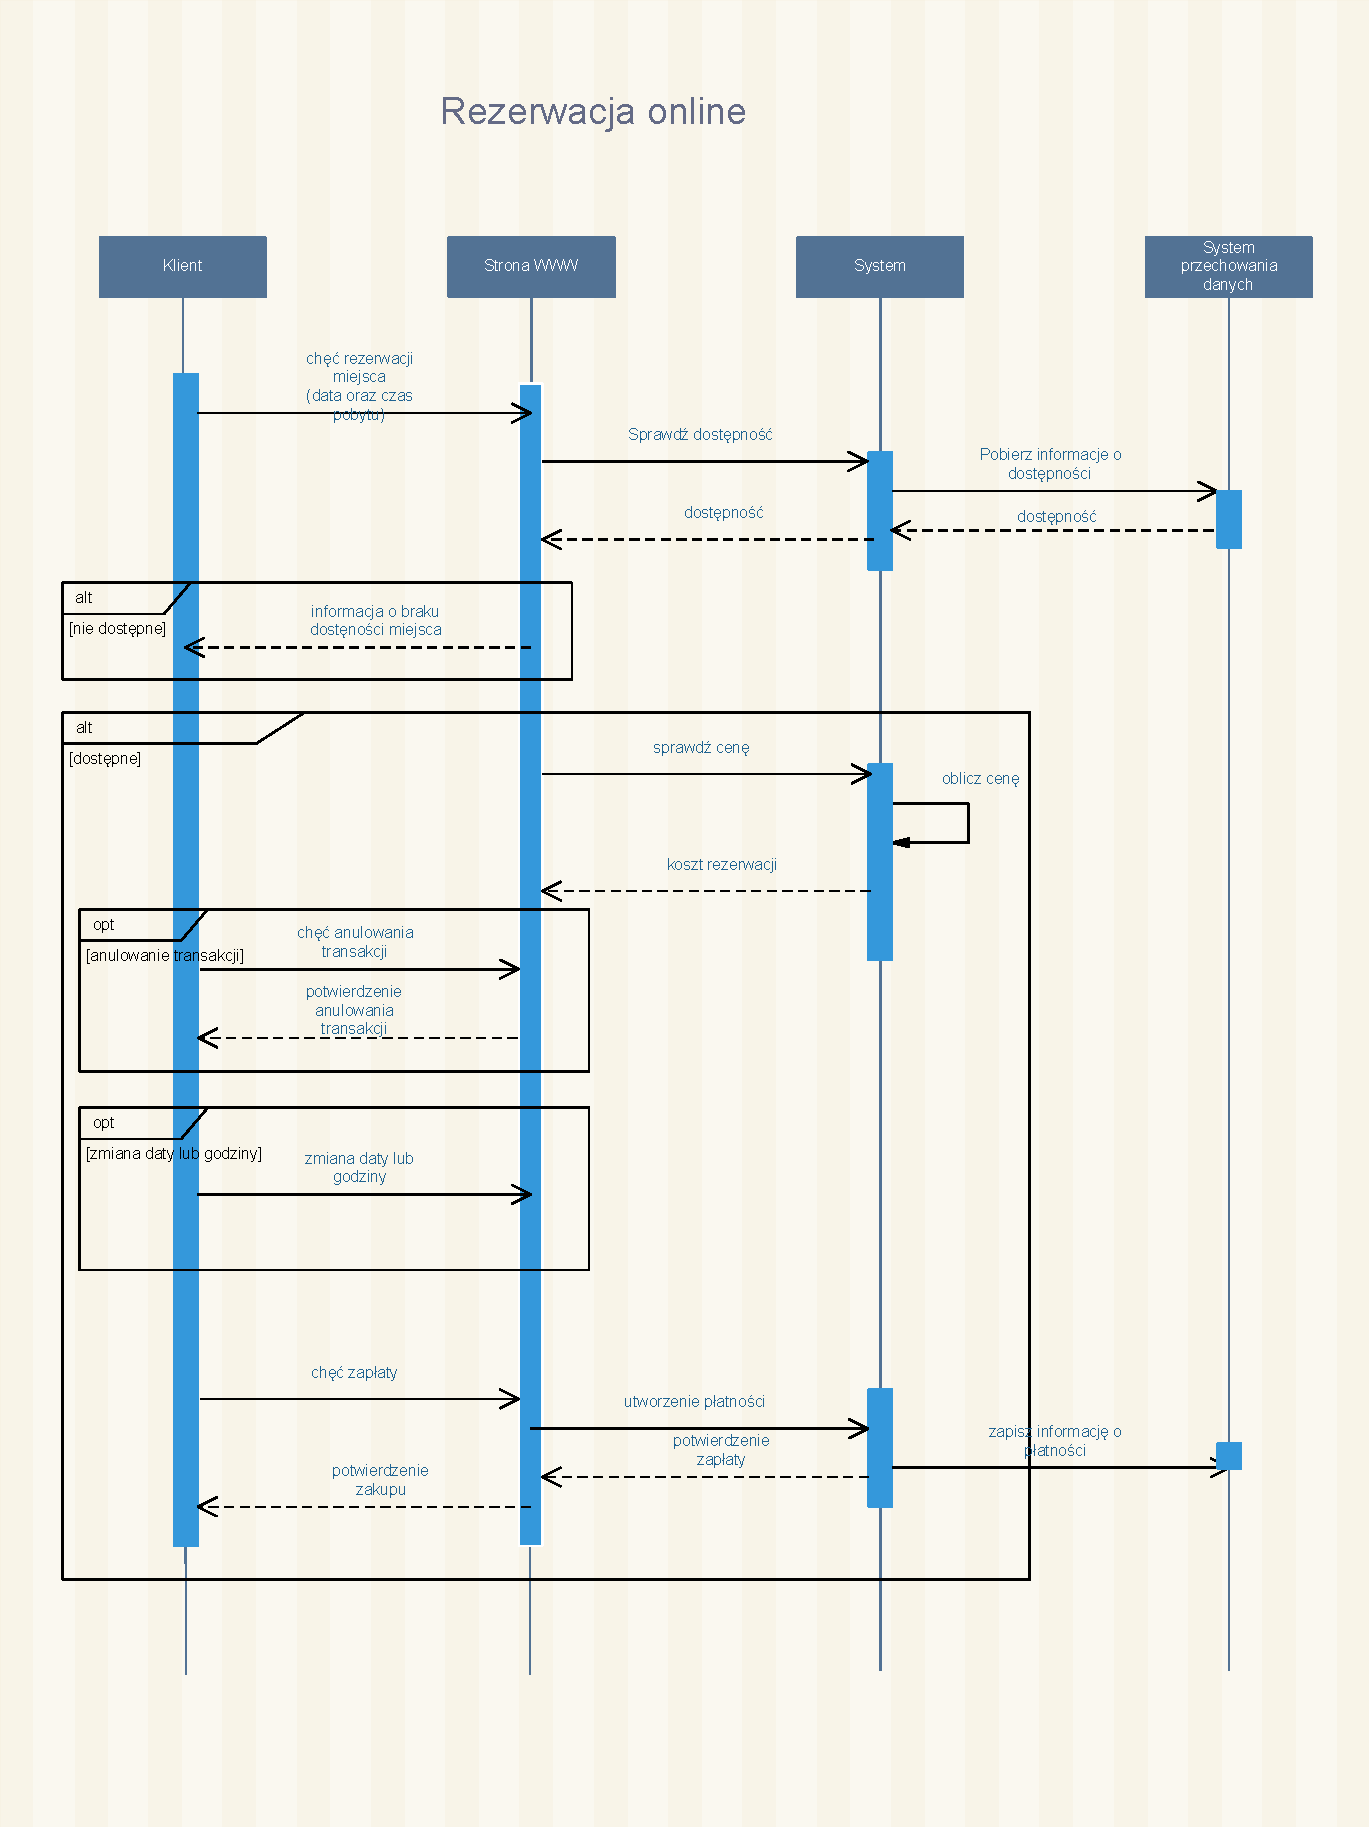
\includepdf[]{sekwencji/rezerwacja-seq}
\newpage
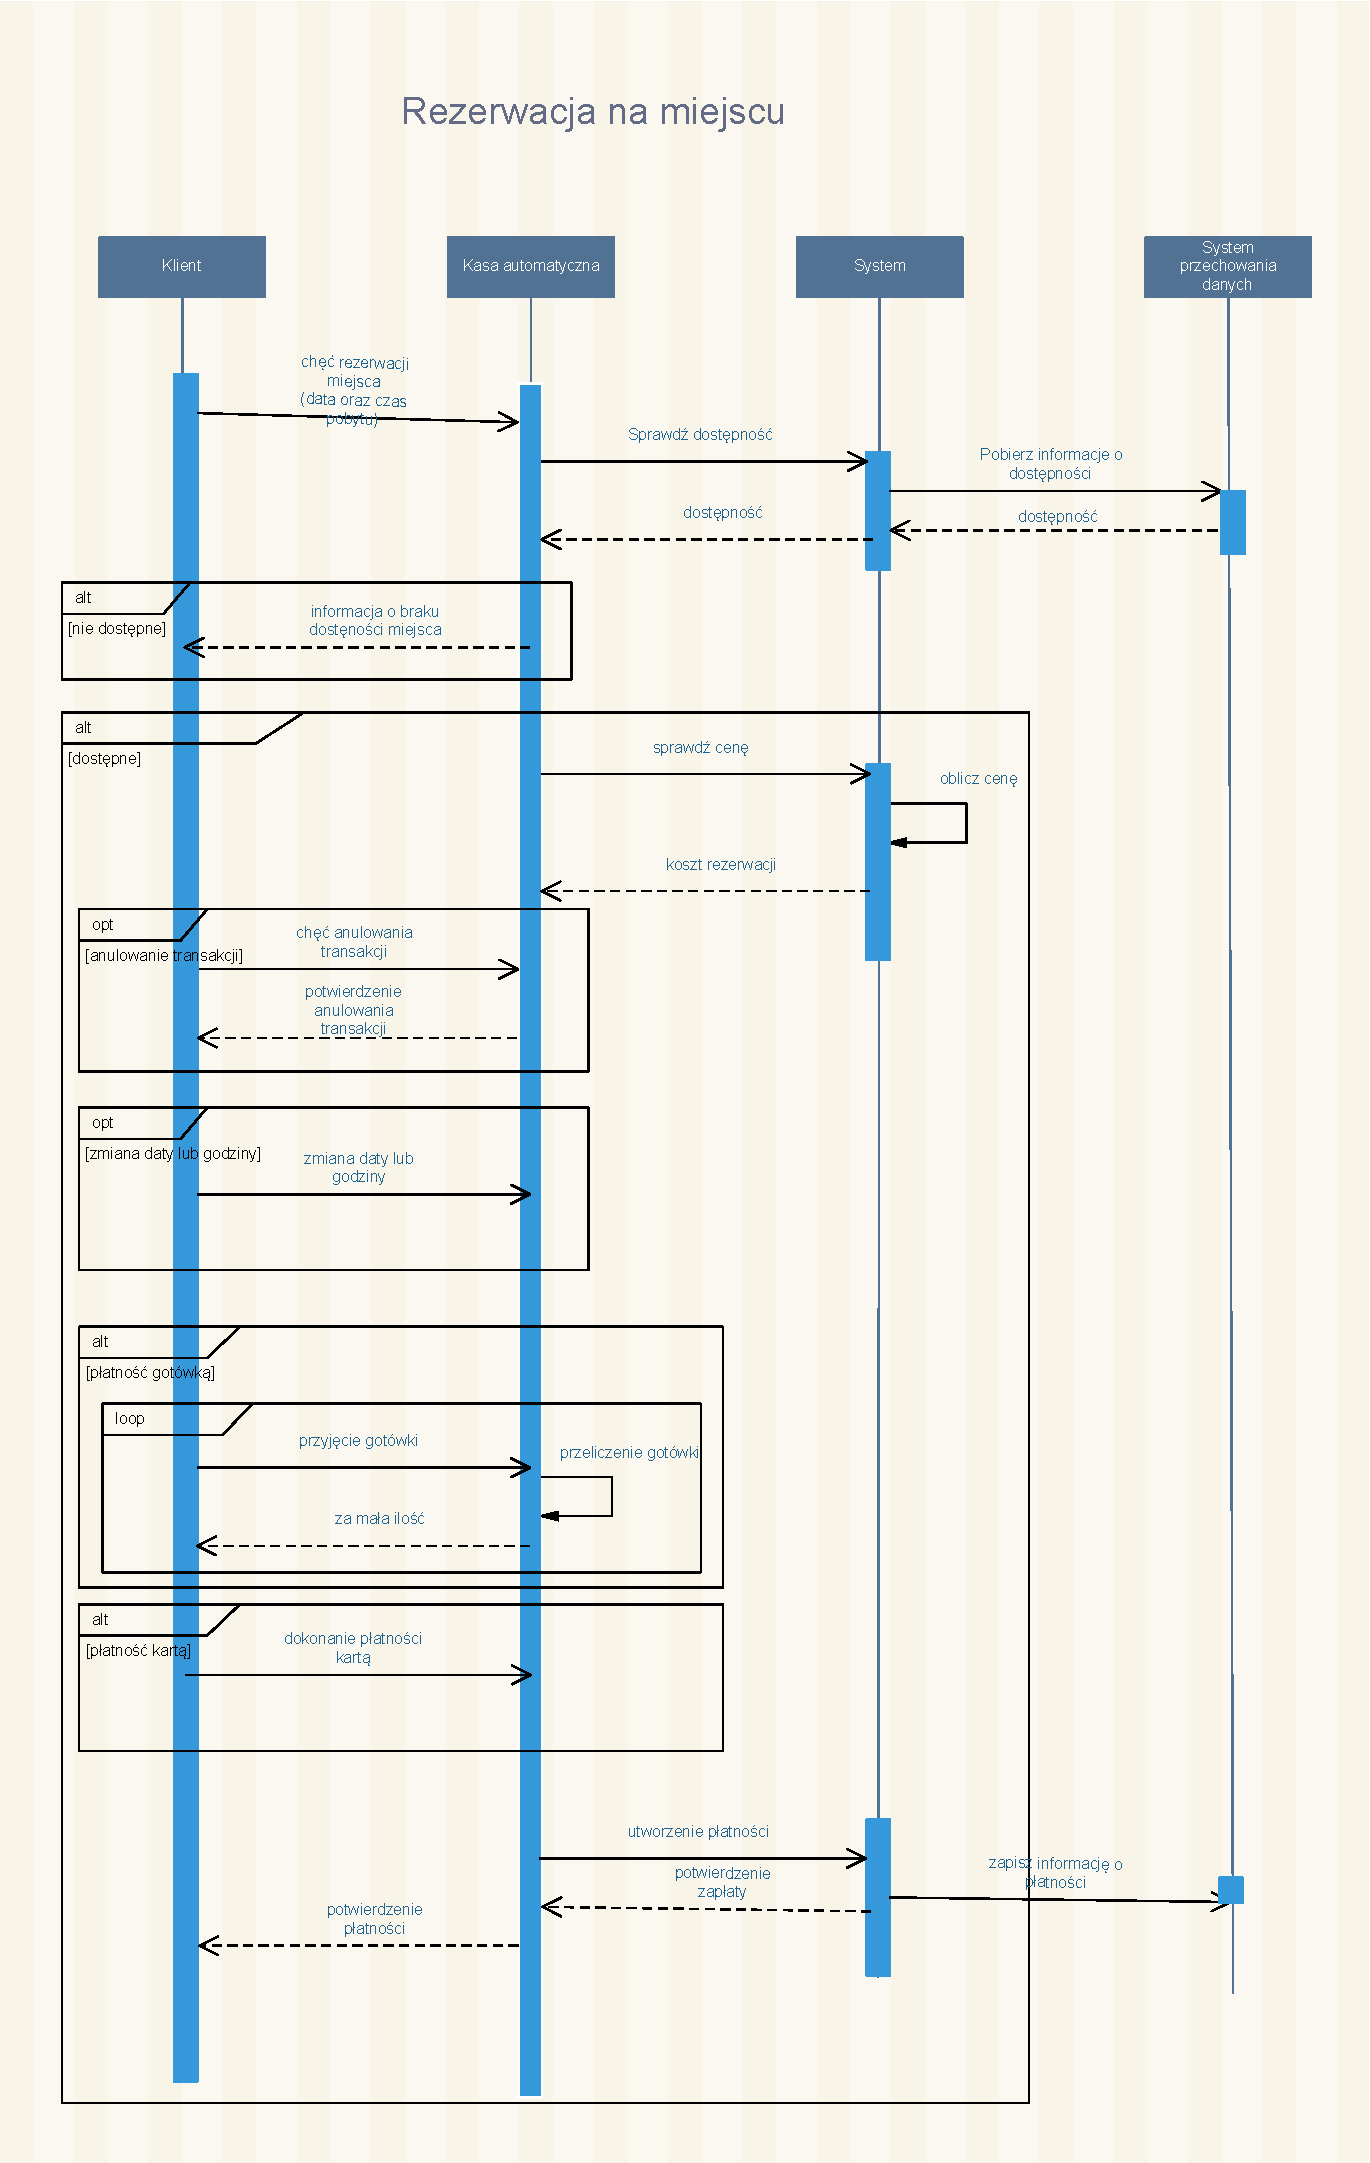
\includepdf[]{sekwencji/rezerwacja2-seq}
\newpage
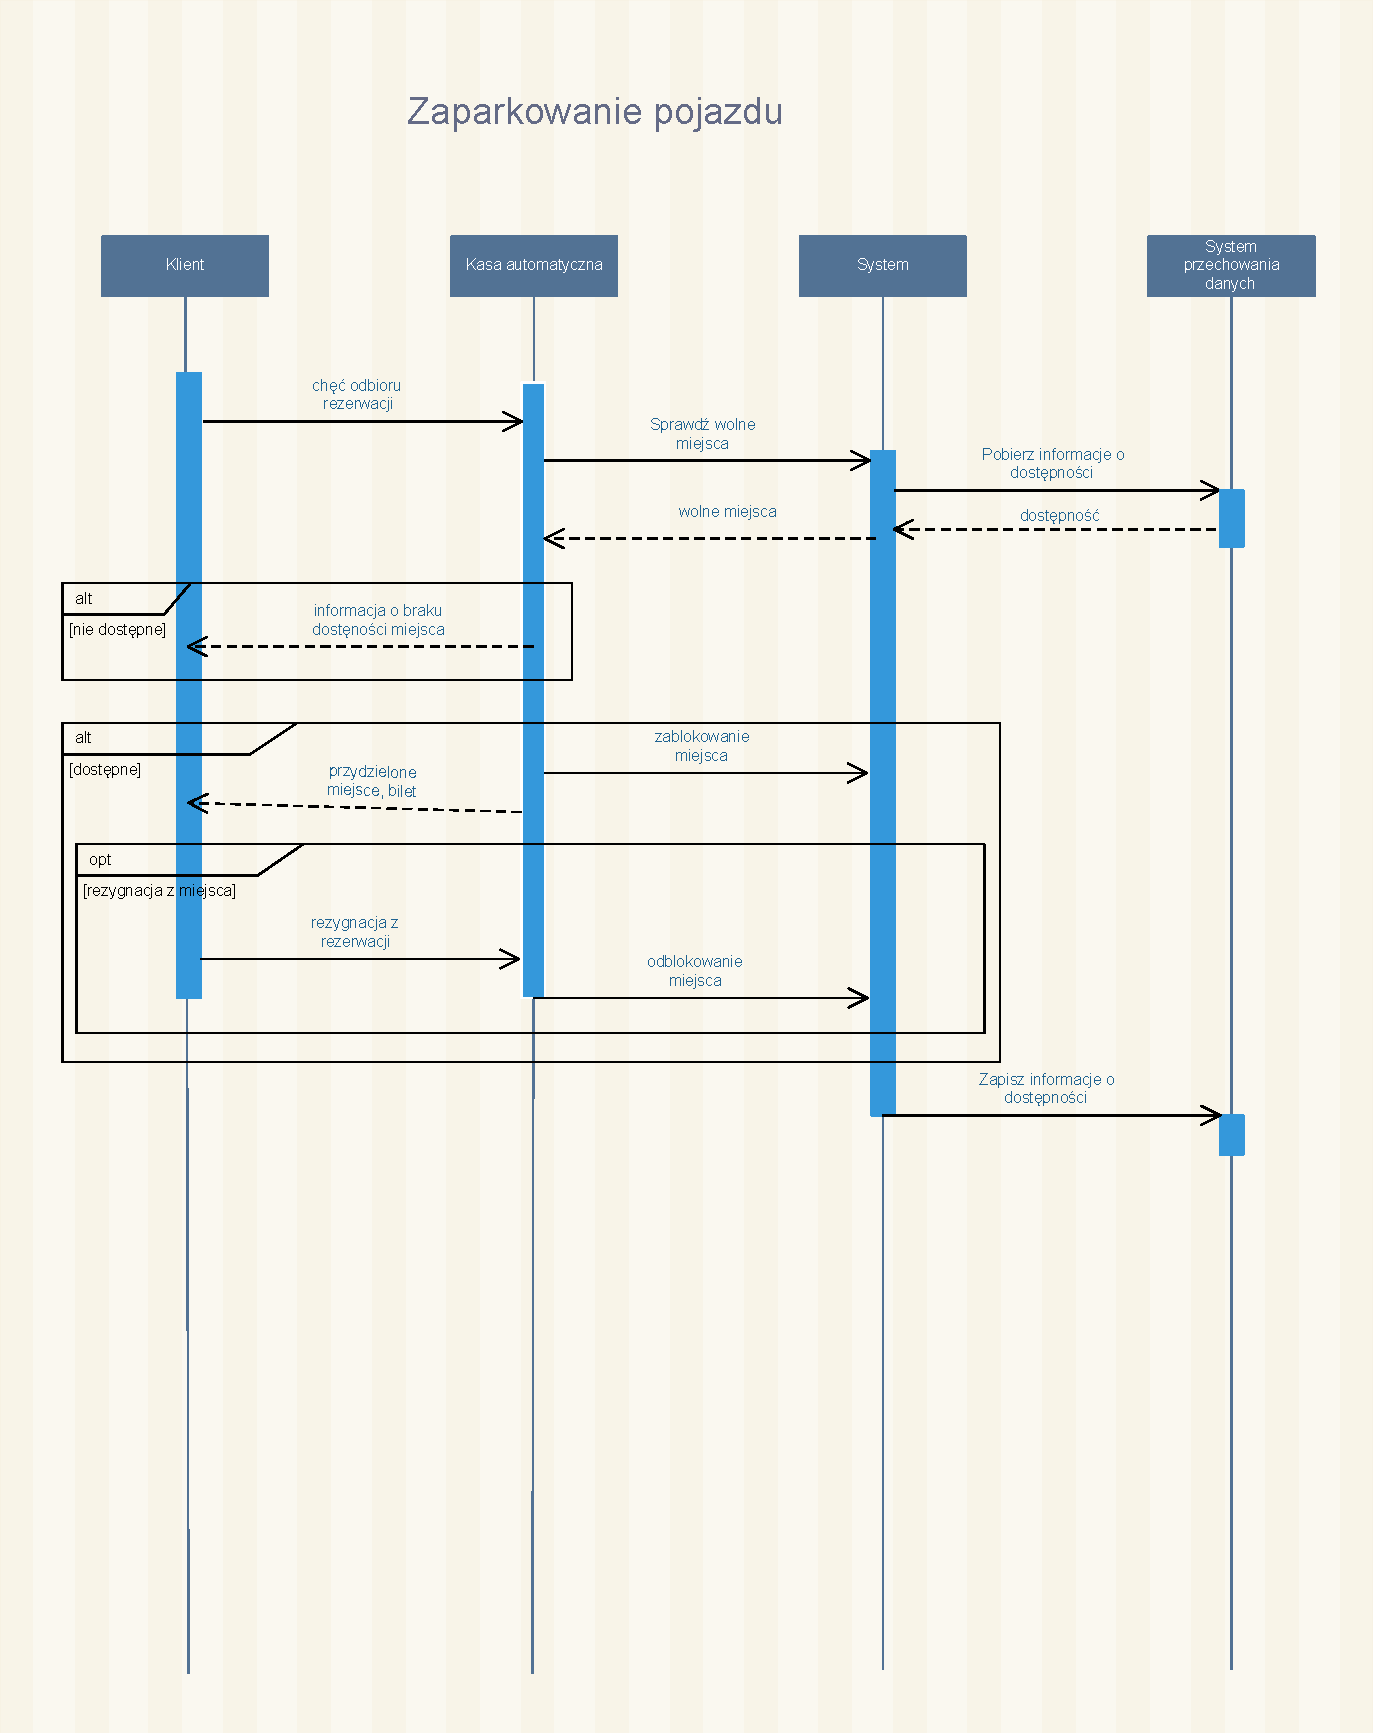
\includepdf[]{sekwencji/parkowanie-seq}
\newpage
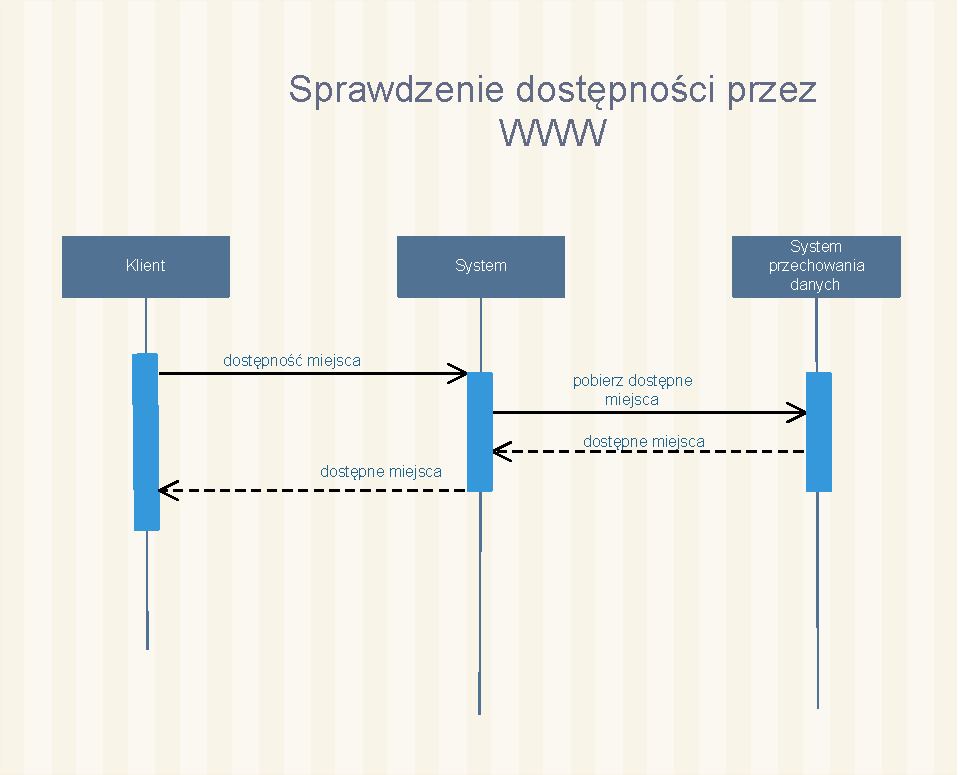
\includepdf[]{sekwencji/dostepnosc}
\newpage
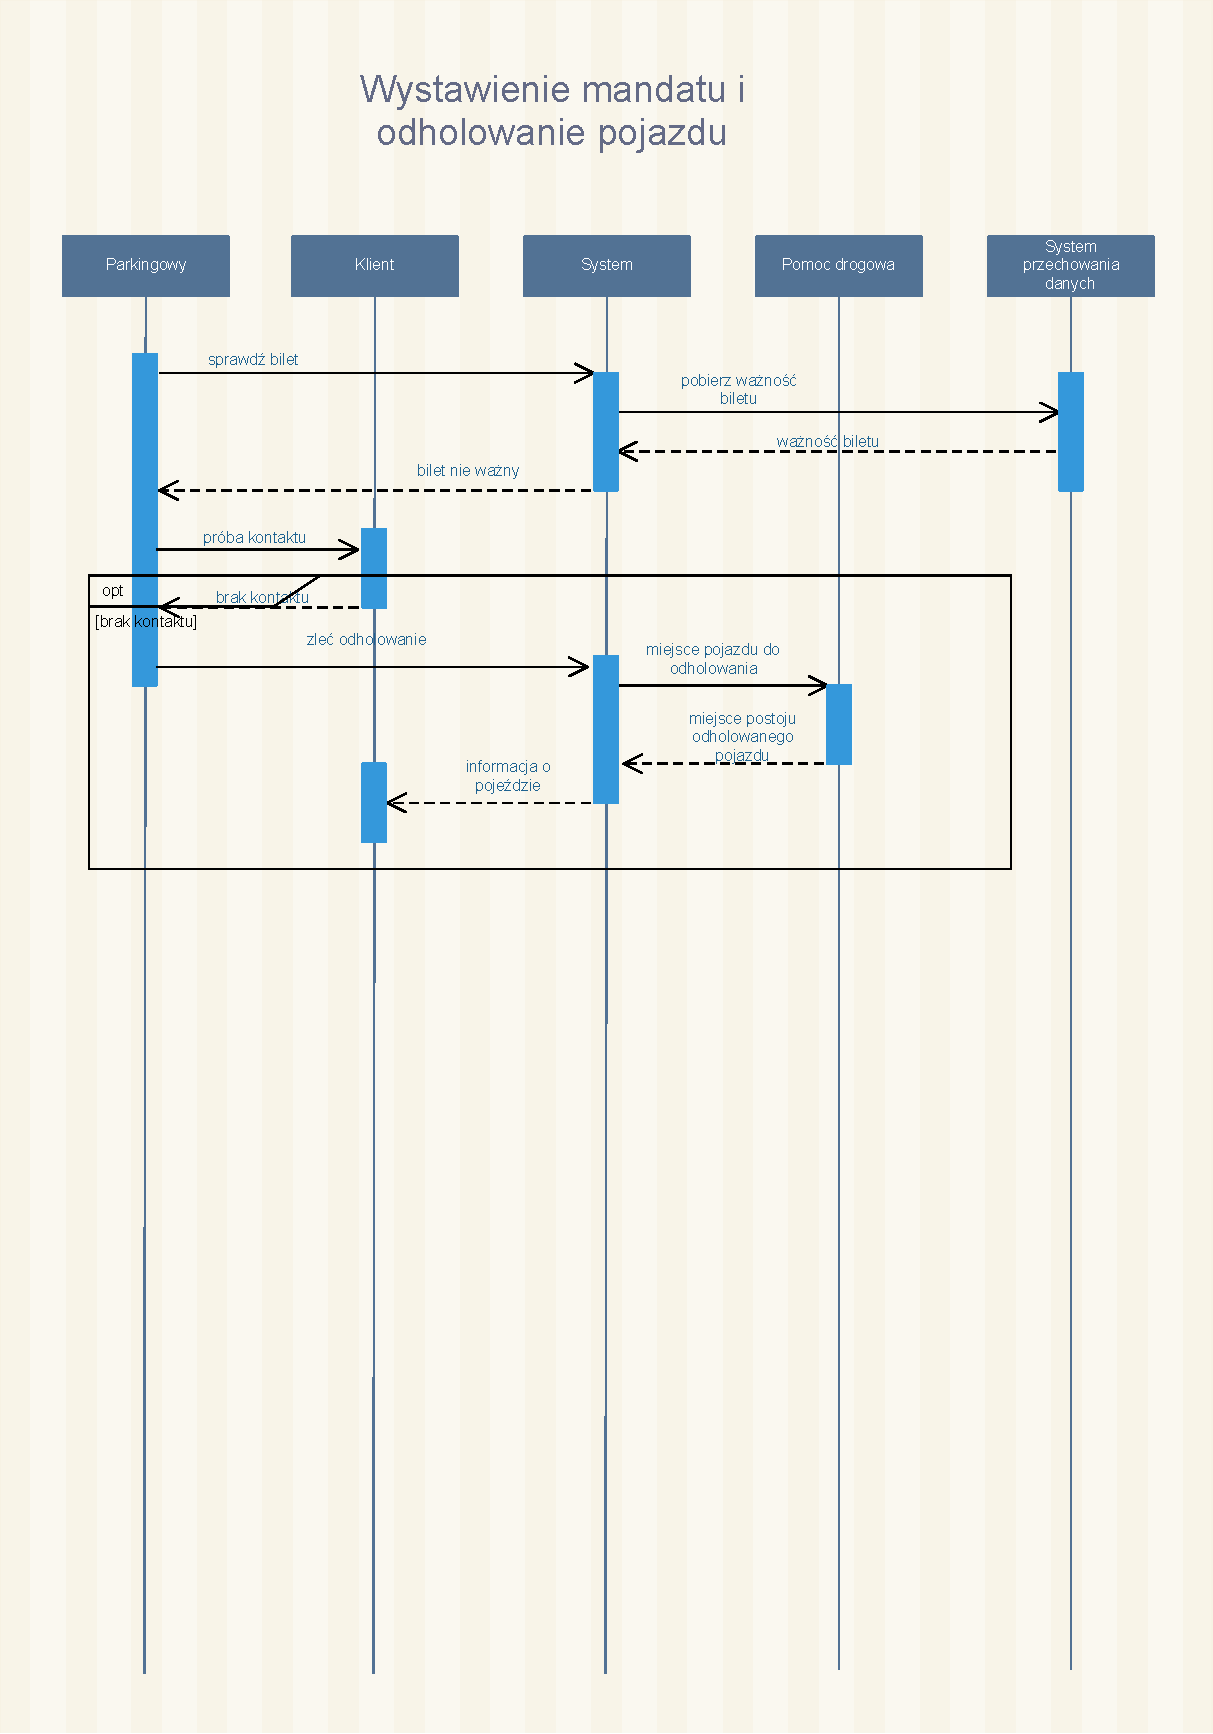
\includepdf[]{sekwencji/odholowanie}
\newpage
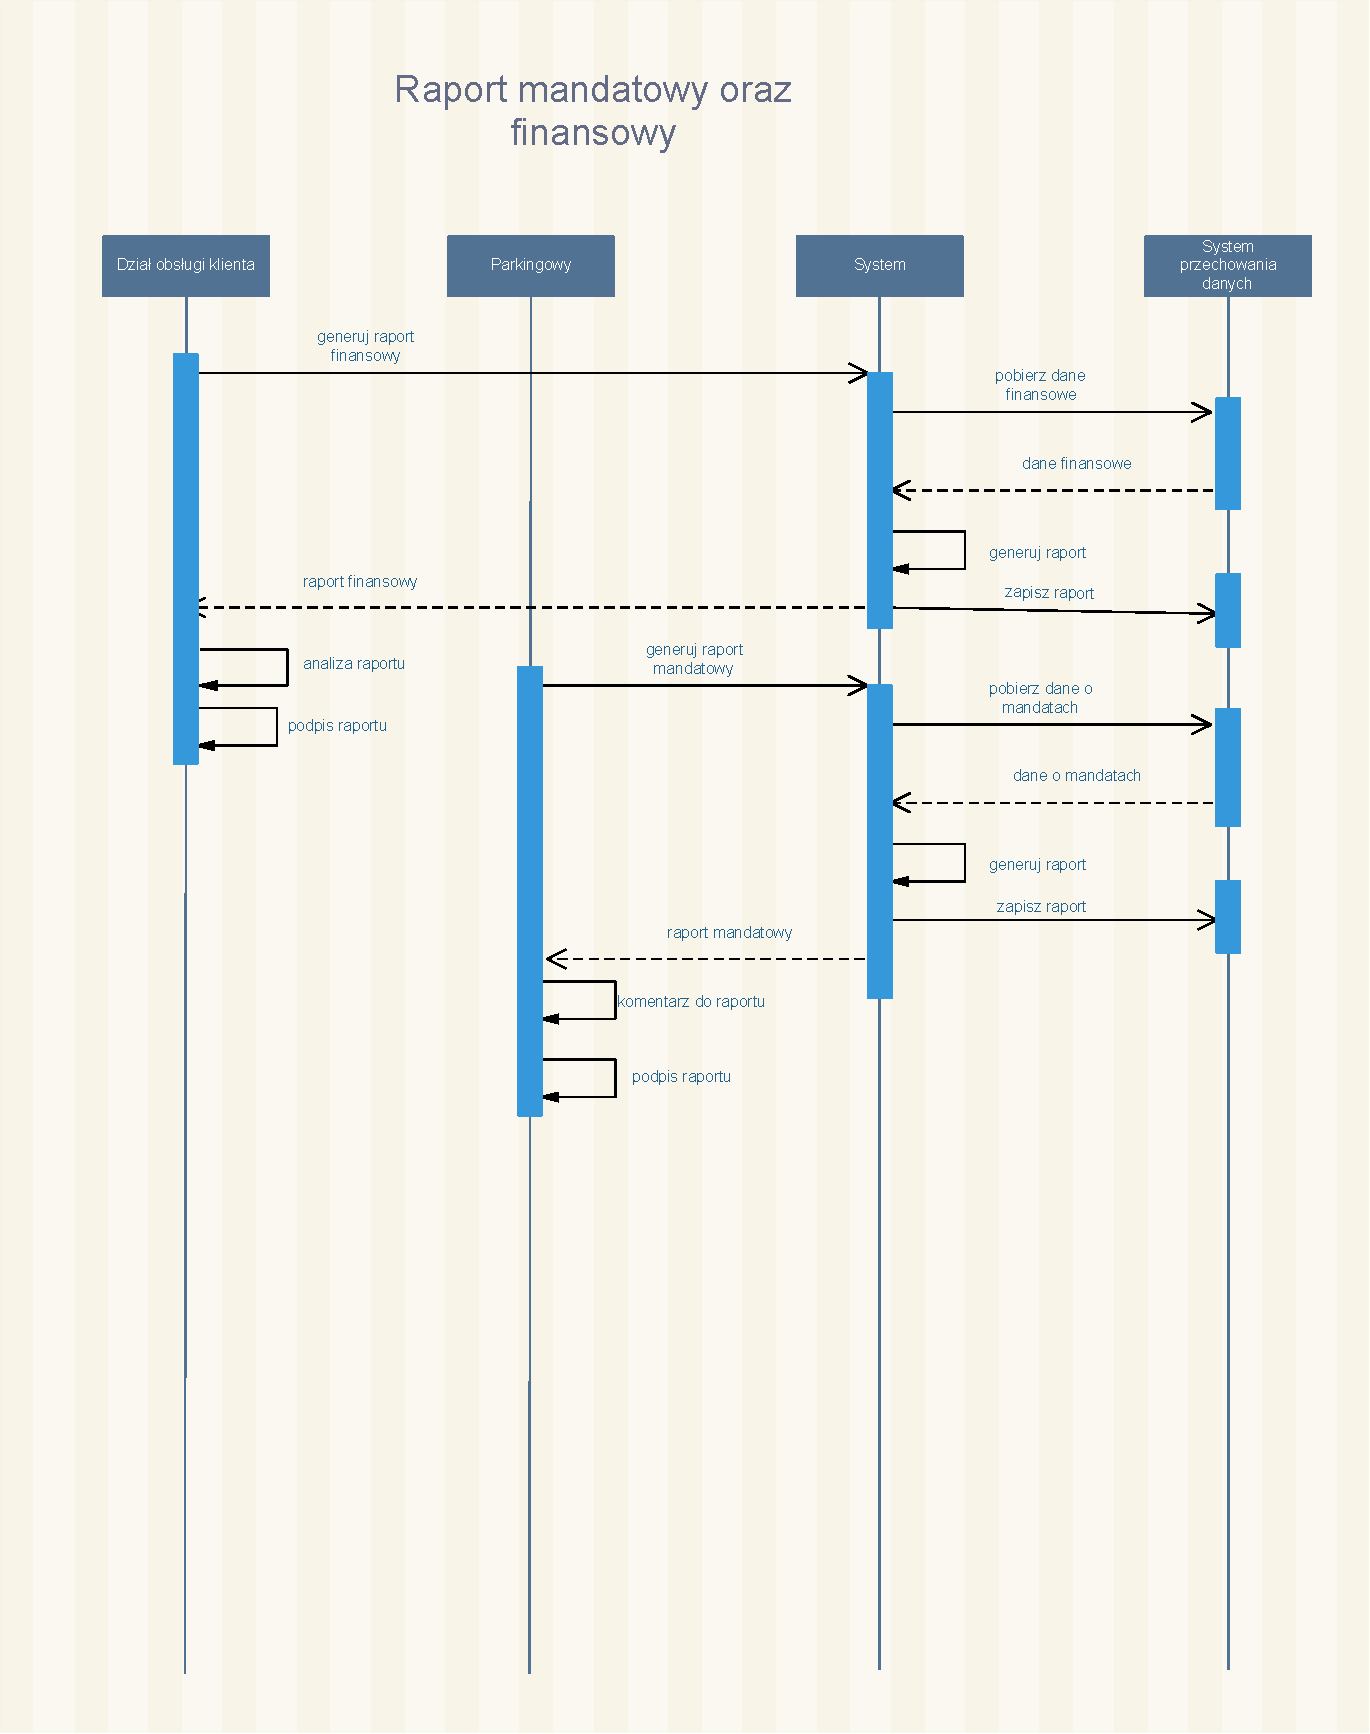
\includepdf[]{sekwencji/raporty}
\newpage
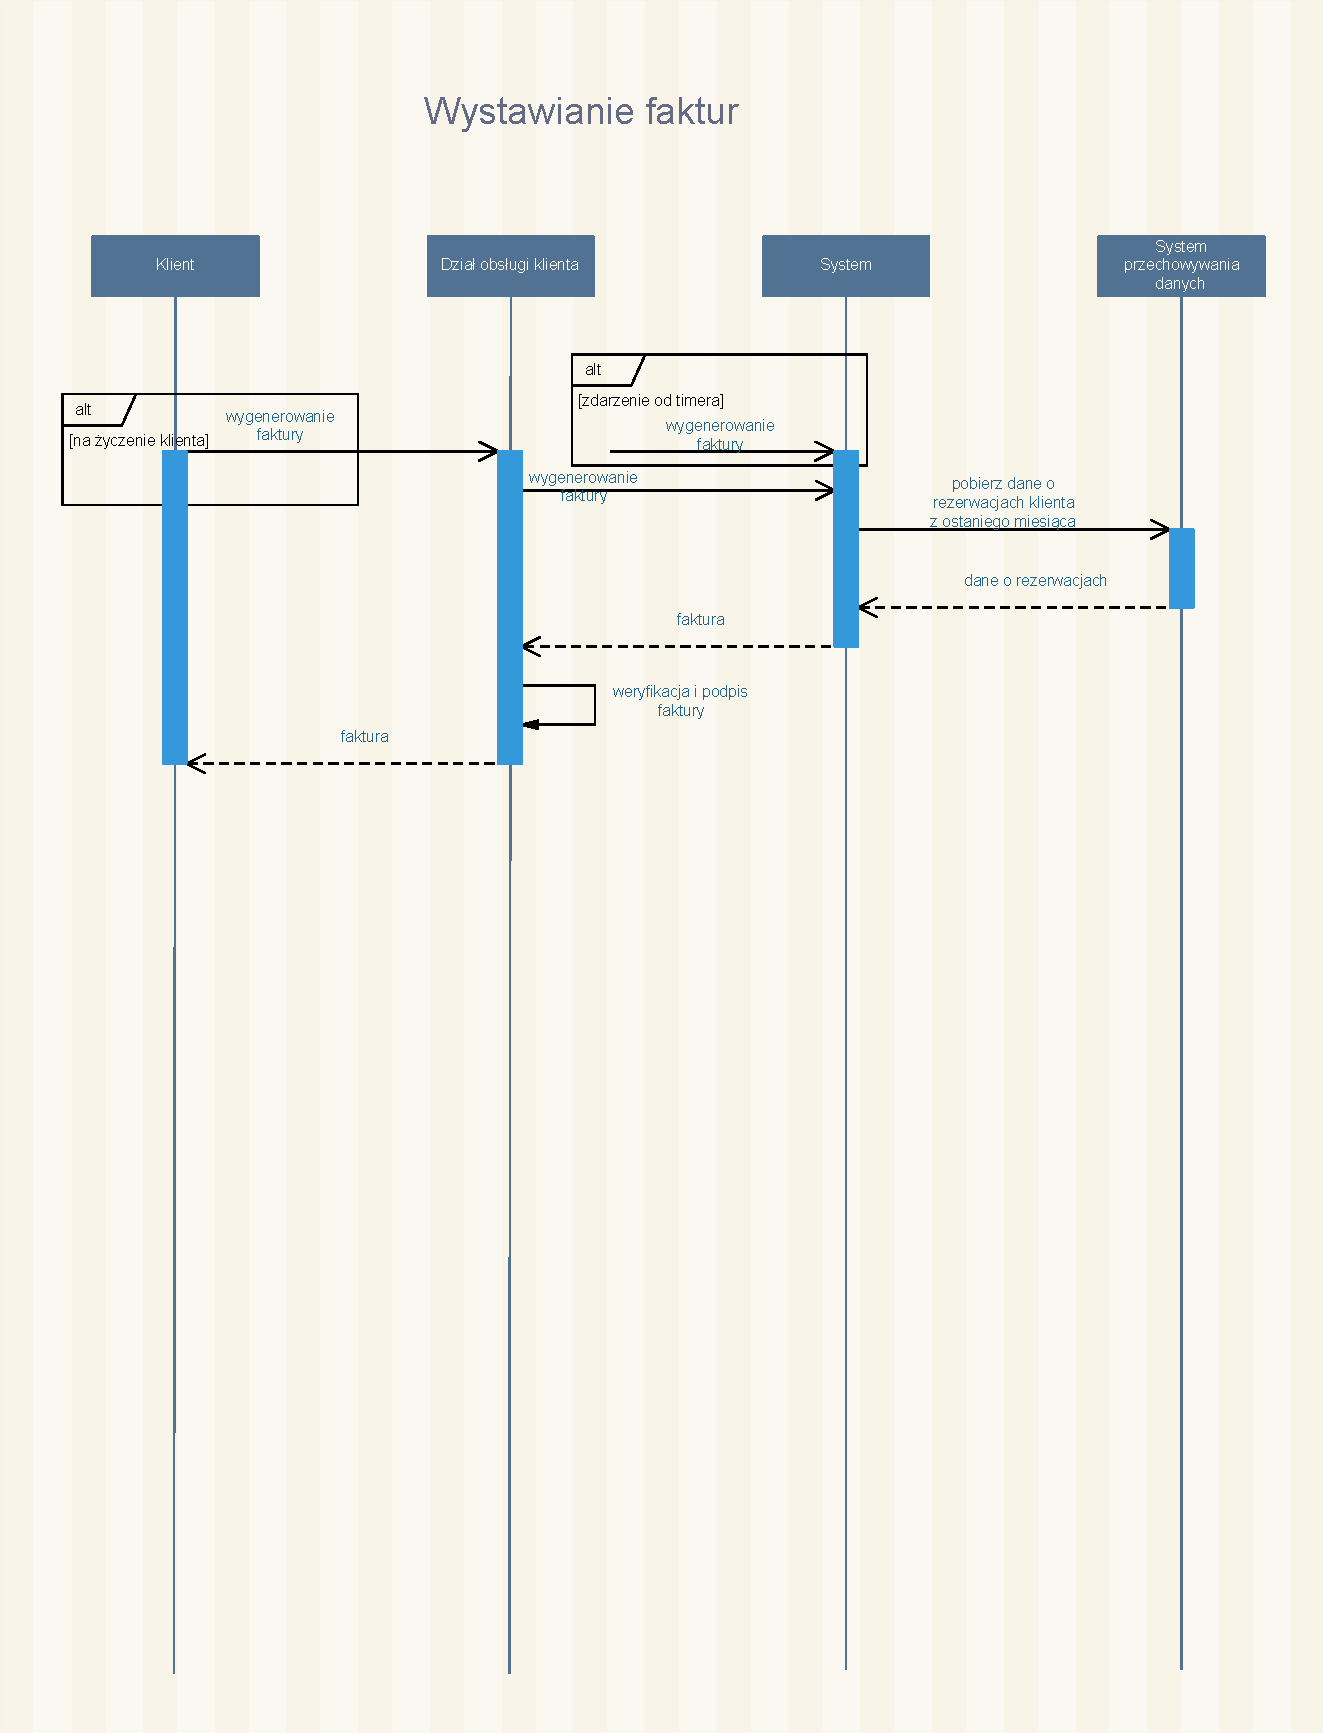
\includepdf[]{sekwencji/faktury}
\newpage
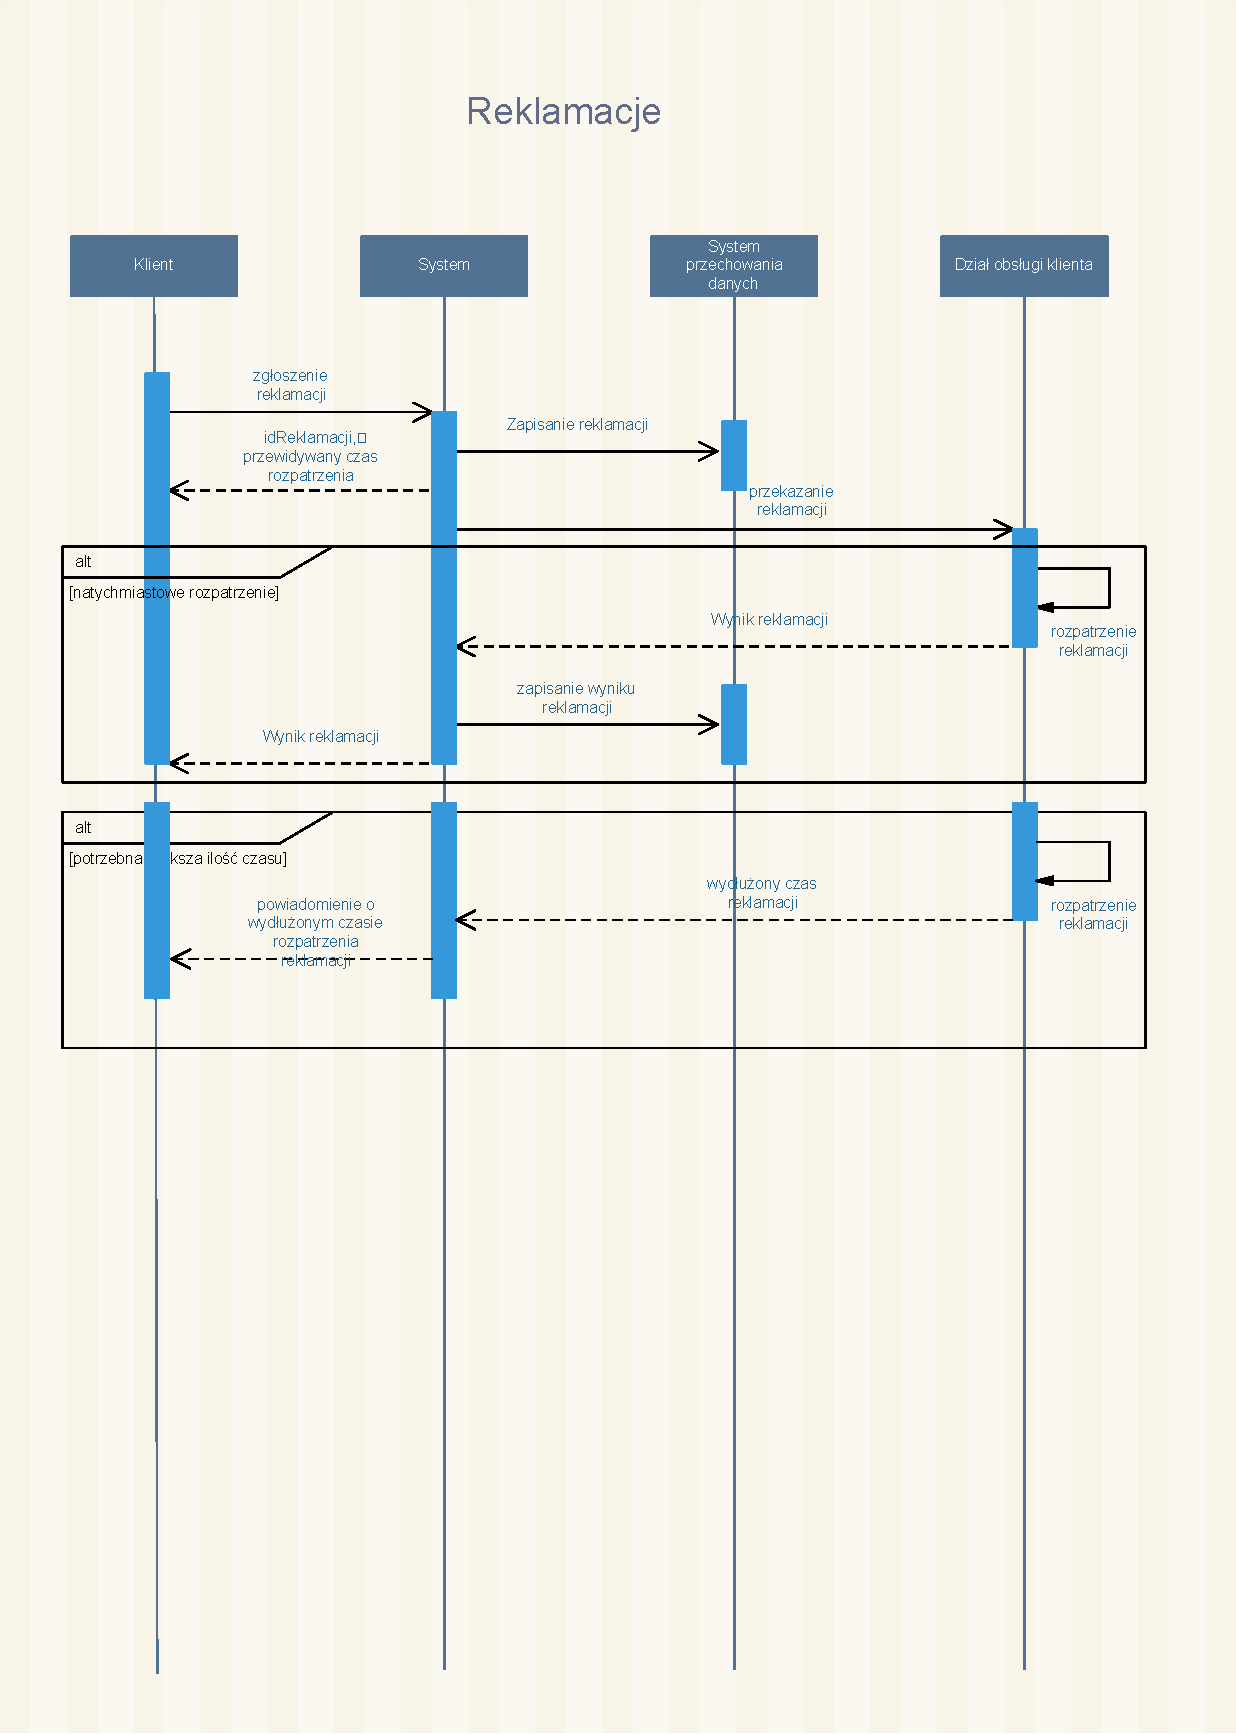
\includepdf[]{sekwencji/reklamacje-seq}
\newpage
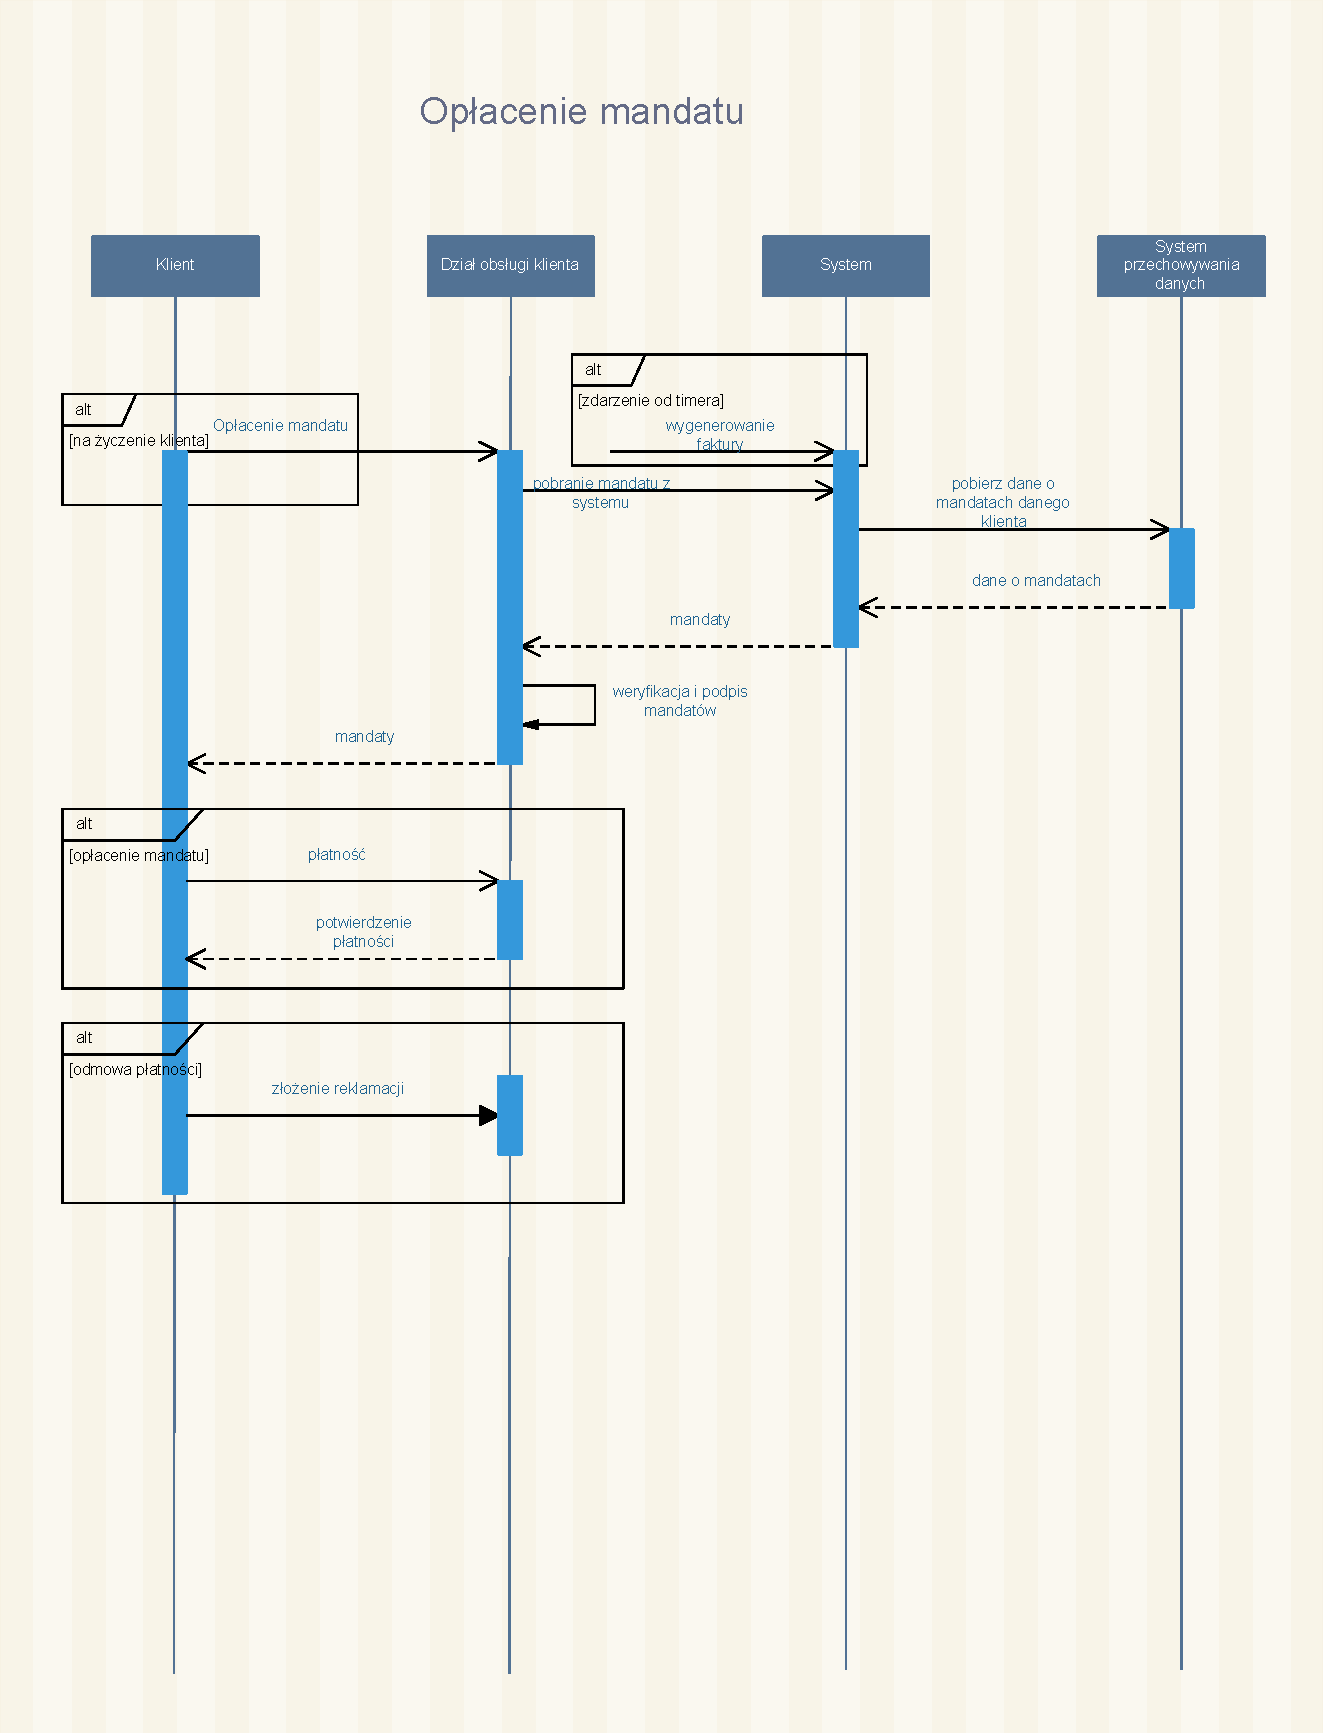
\includepdf[]{sekwencji/mandaty}
\end{center}
\newpage
\section{Diagramy aktywności}
\subsection{Rezerwacja zdalna}
\subsection{Obsługa płatności}
\subsection{Ważność rezerwacji}
\subsection{Rezerwacja na miejscu}
\subsection{Parkowanie}
\subsection{Generowanie raportu}
\newpage
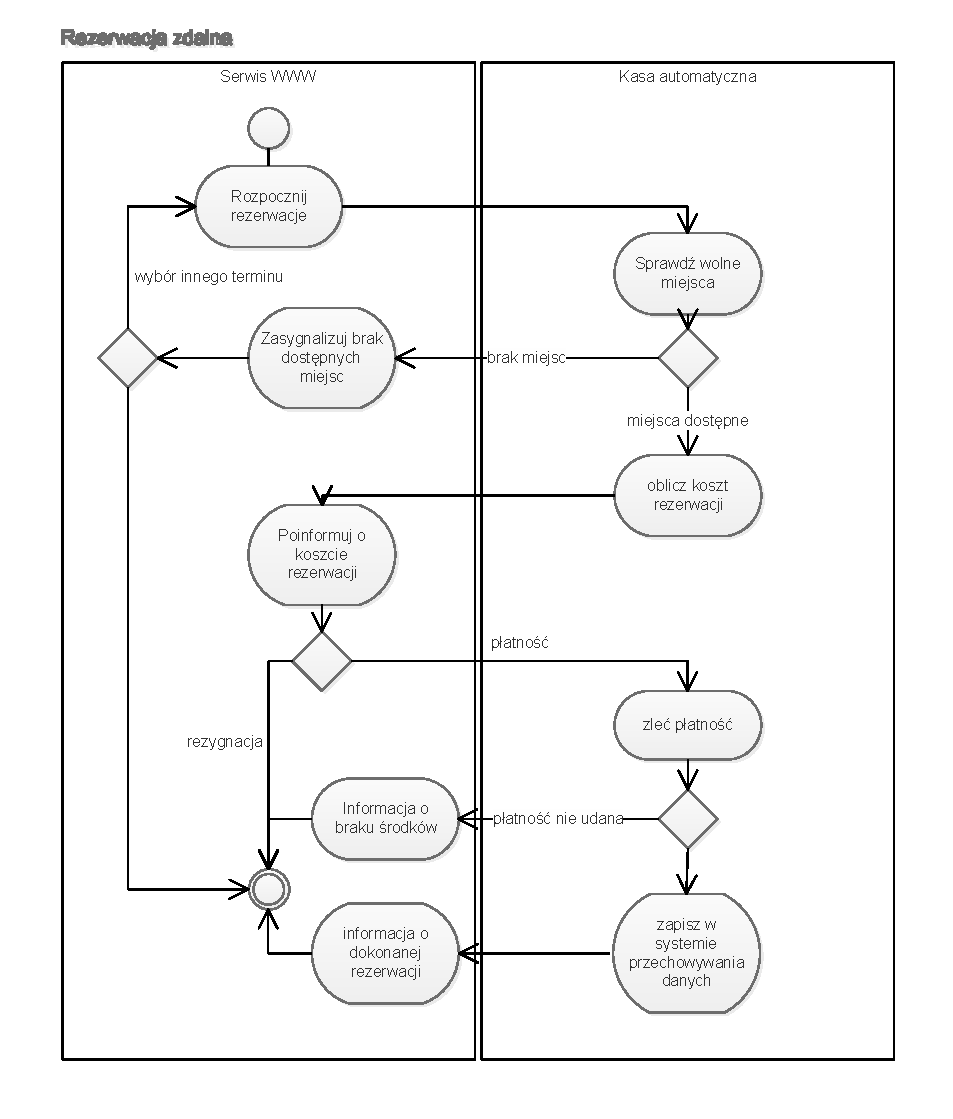
\includepdf[]{aktywnosci/aktywnosci-1}
\newpage
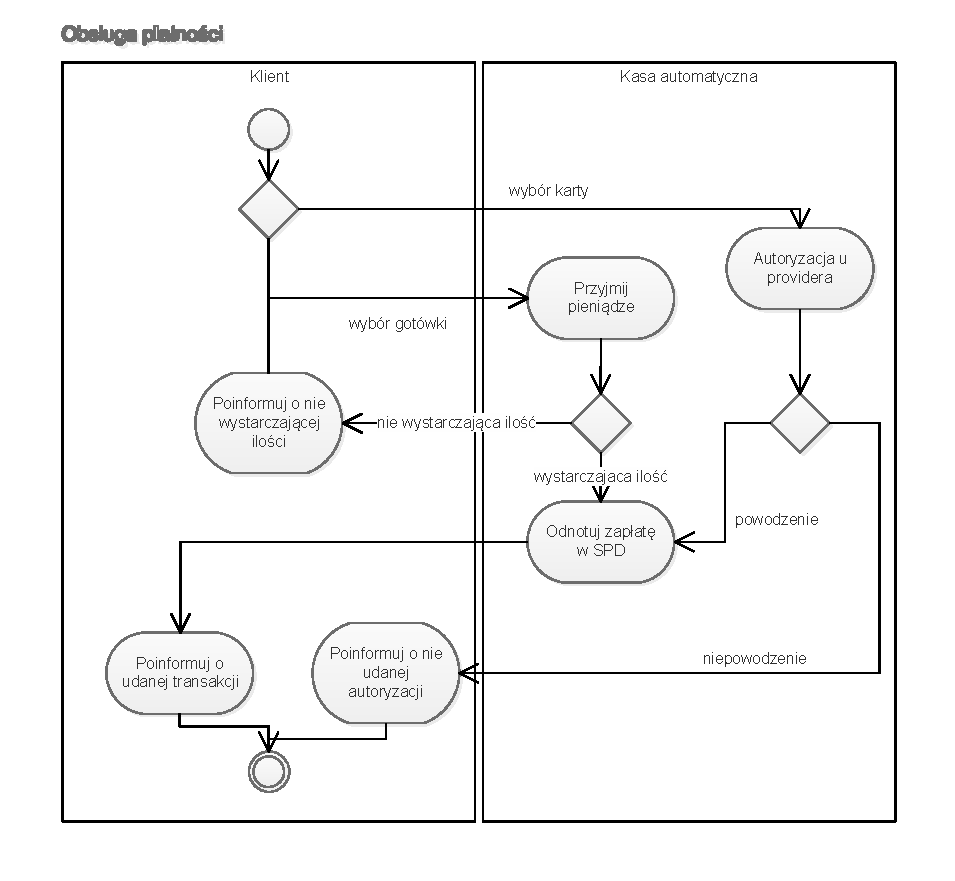
\includepdf[]{aktywnosci/aktywnosci-2}
\newpage
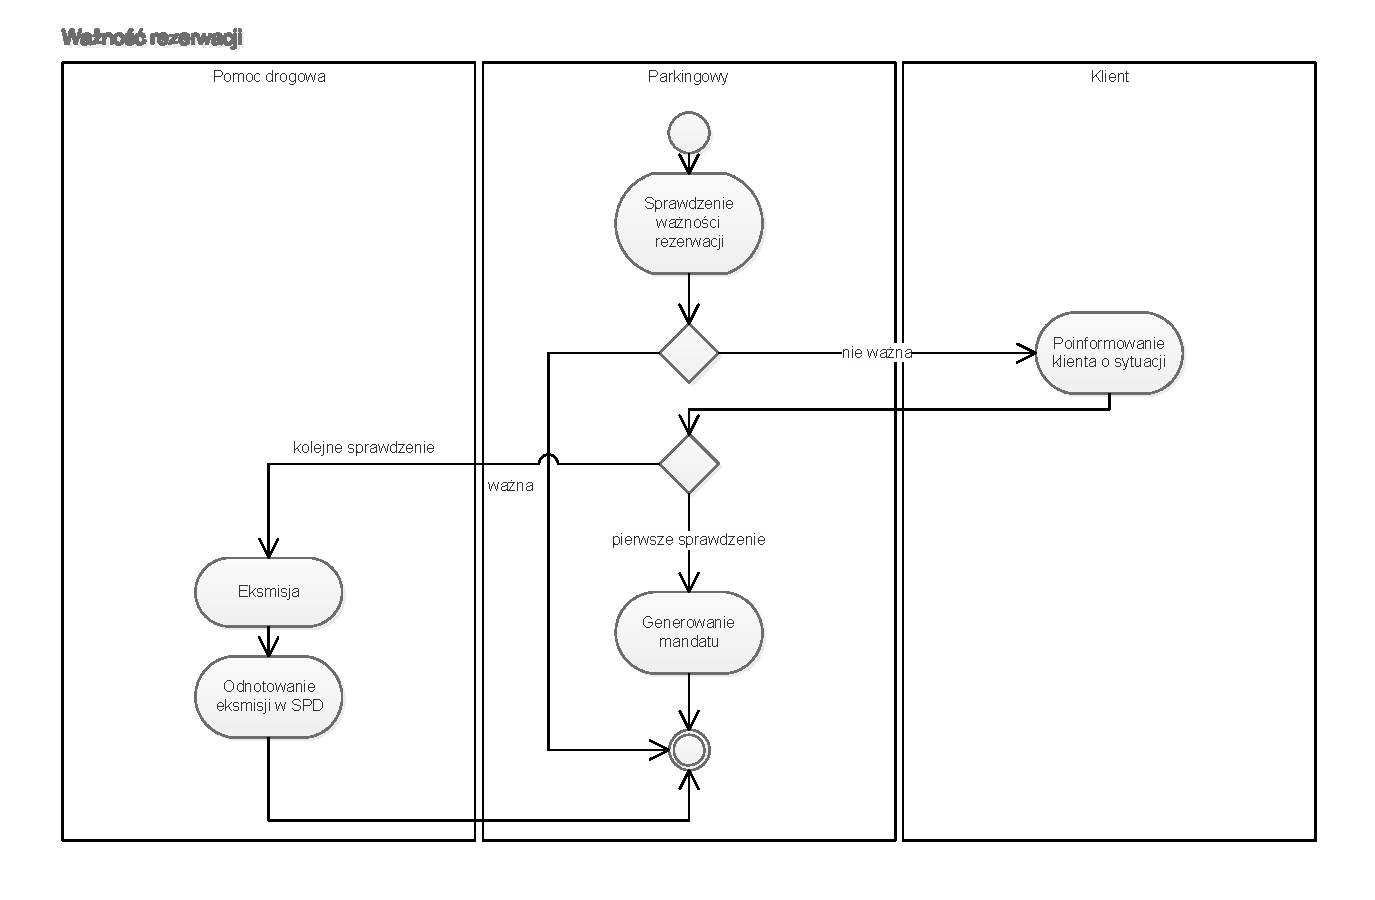
\includepdf[]{aktywnosci/aktywnosci-3}
\newpage
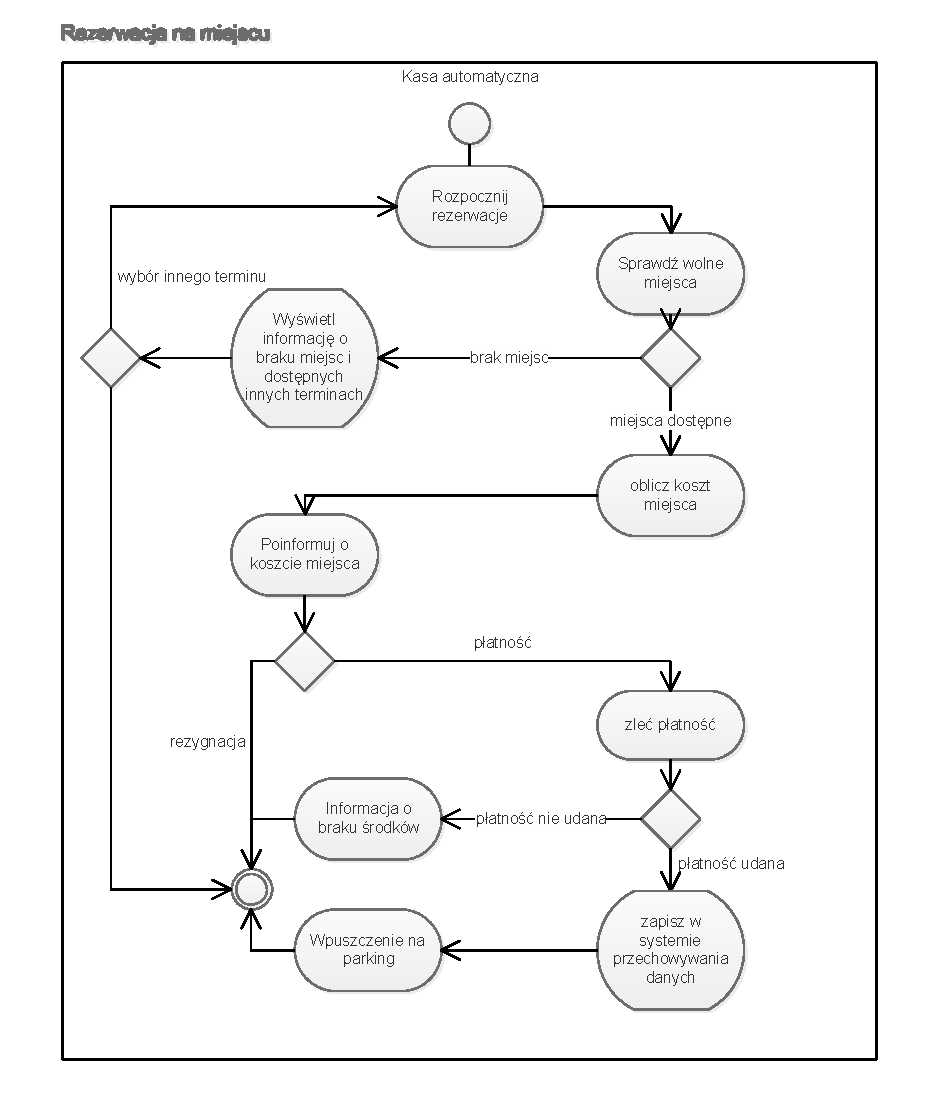
\includepdf[]{aktywnosci/aktywnosci-4}
\newpage
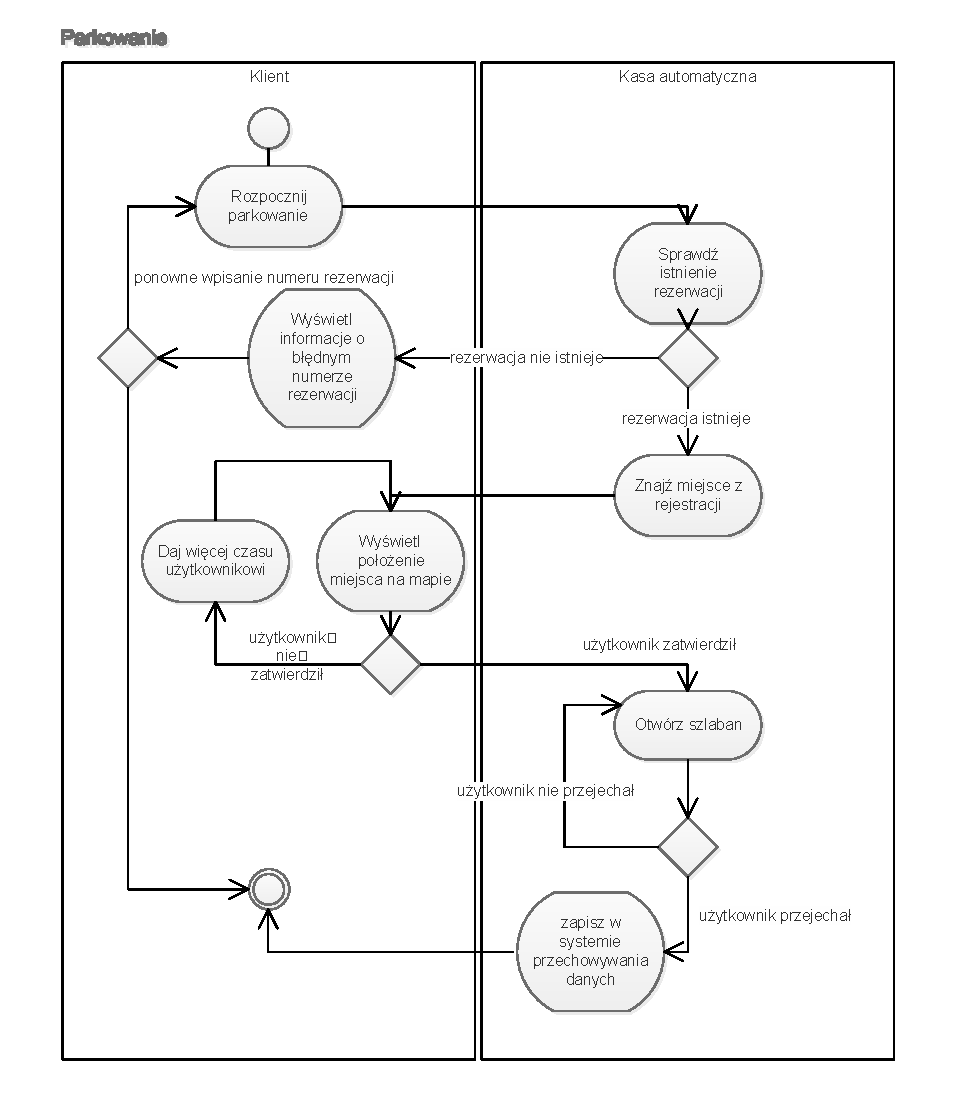
\includepdf[]{aktywnosci/aktywnosci-5}
\newpage
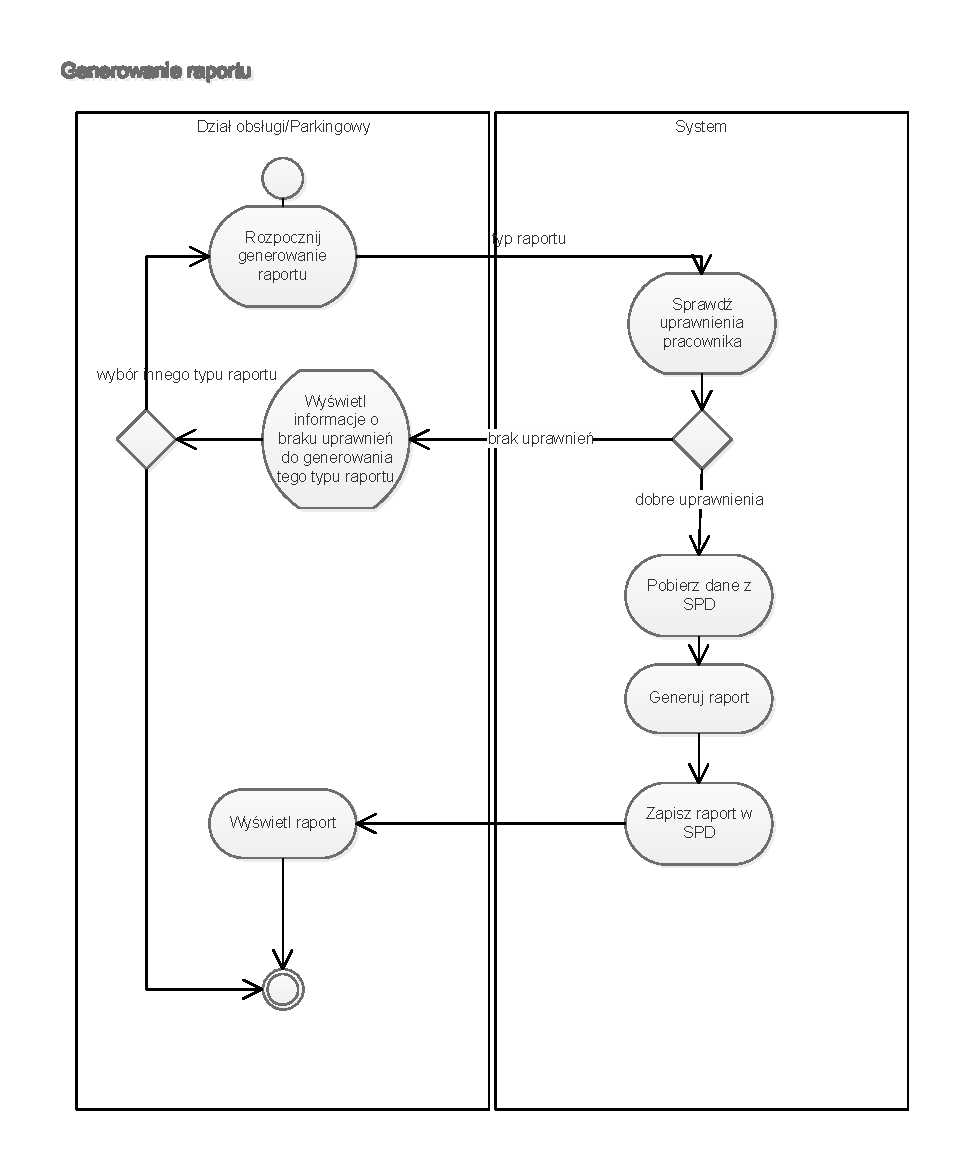
\includepdf[]{aktywnosci/aktywnosci-6}
\newpage
\section{Diagram klas}
\begin{figure}
  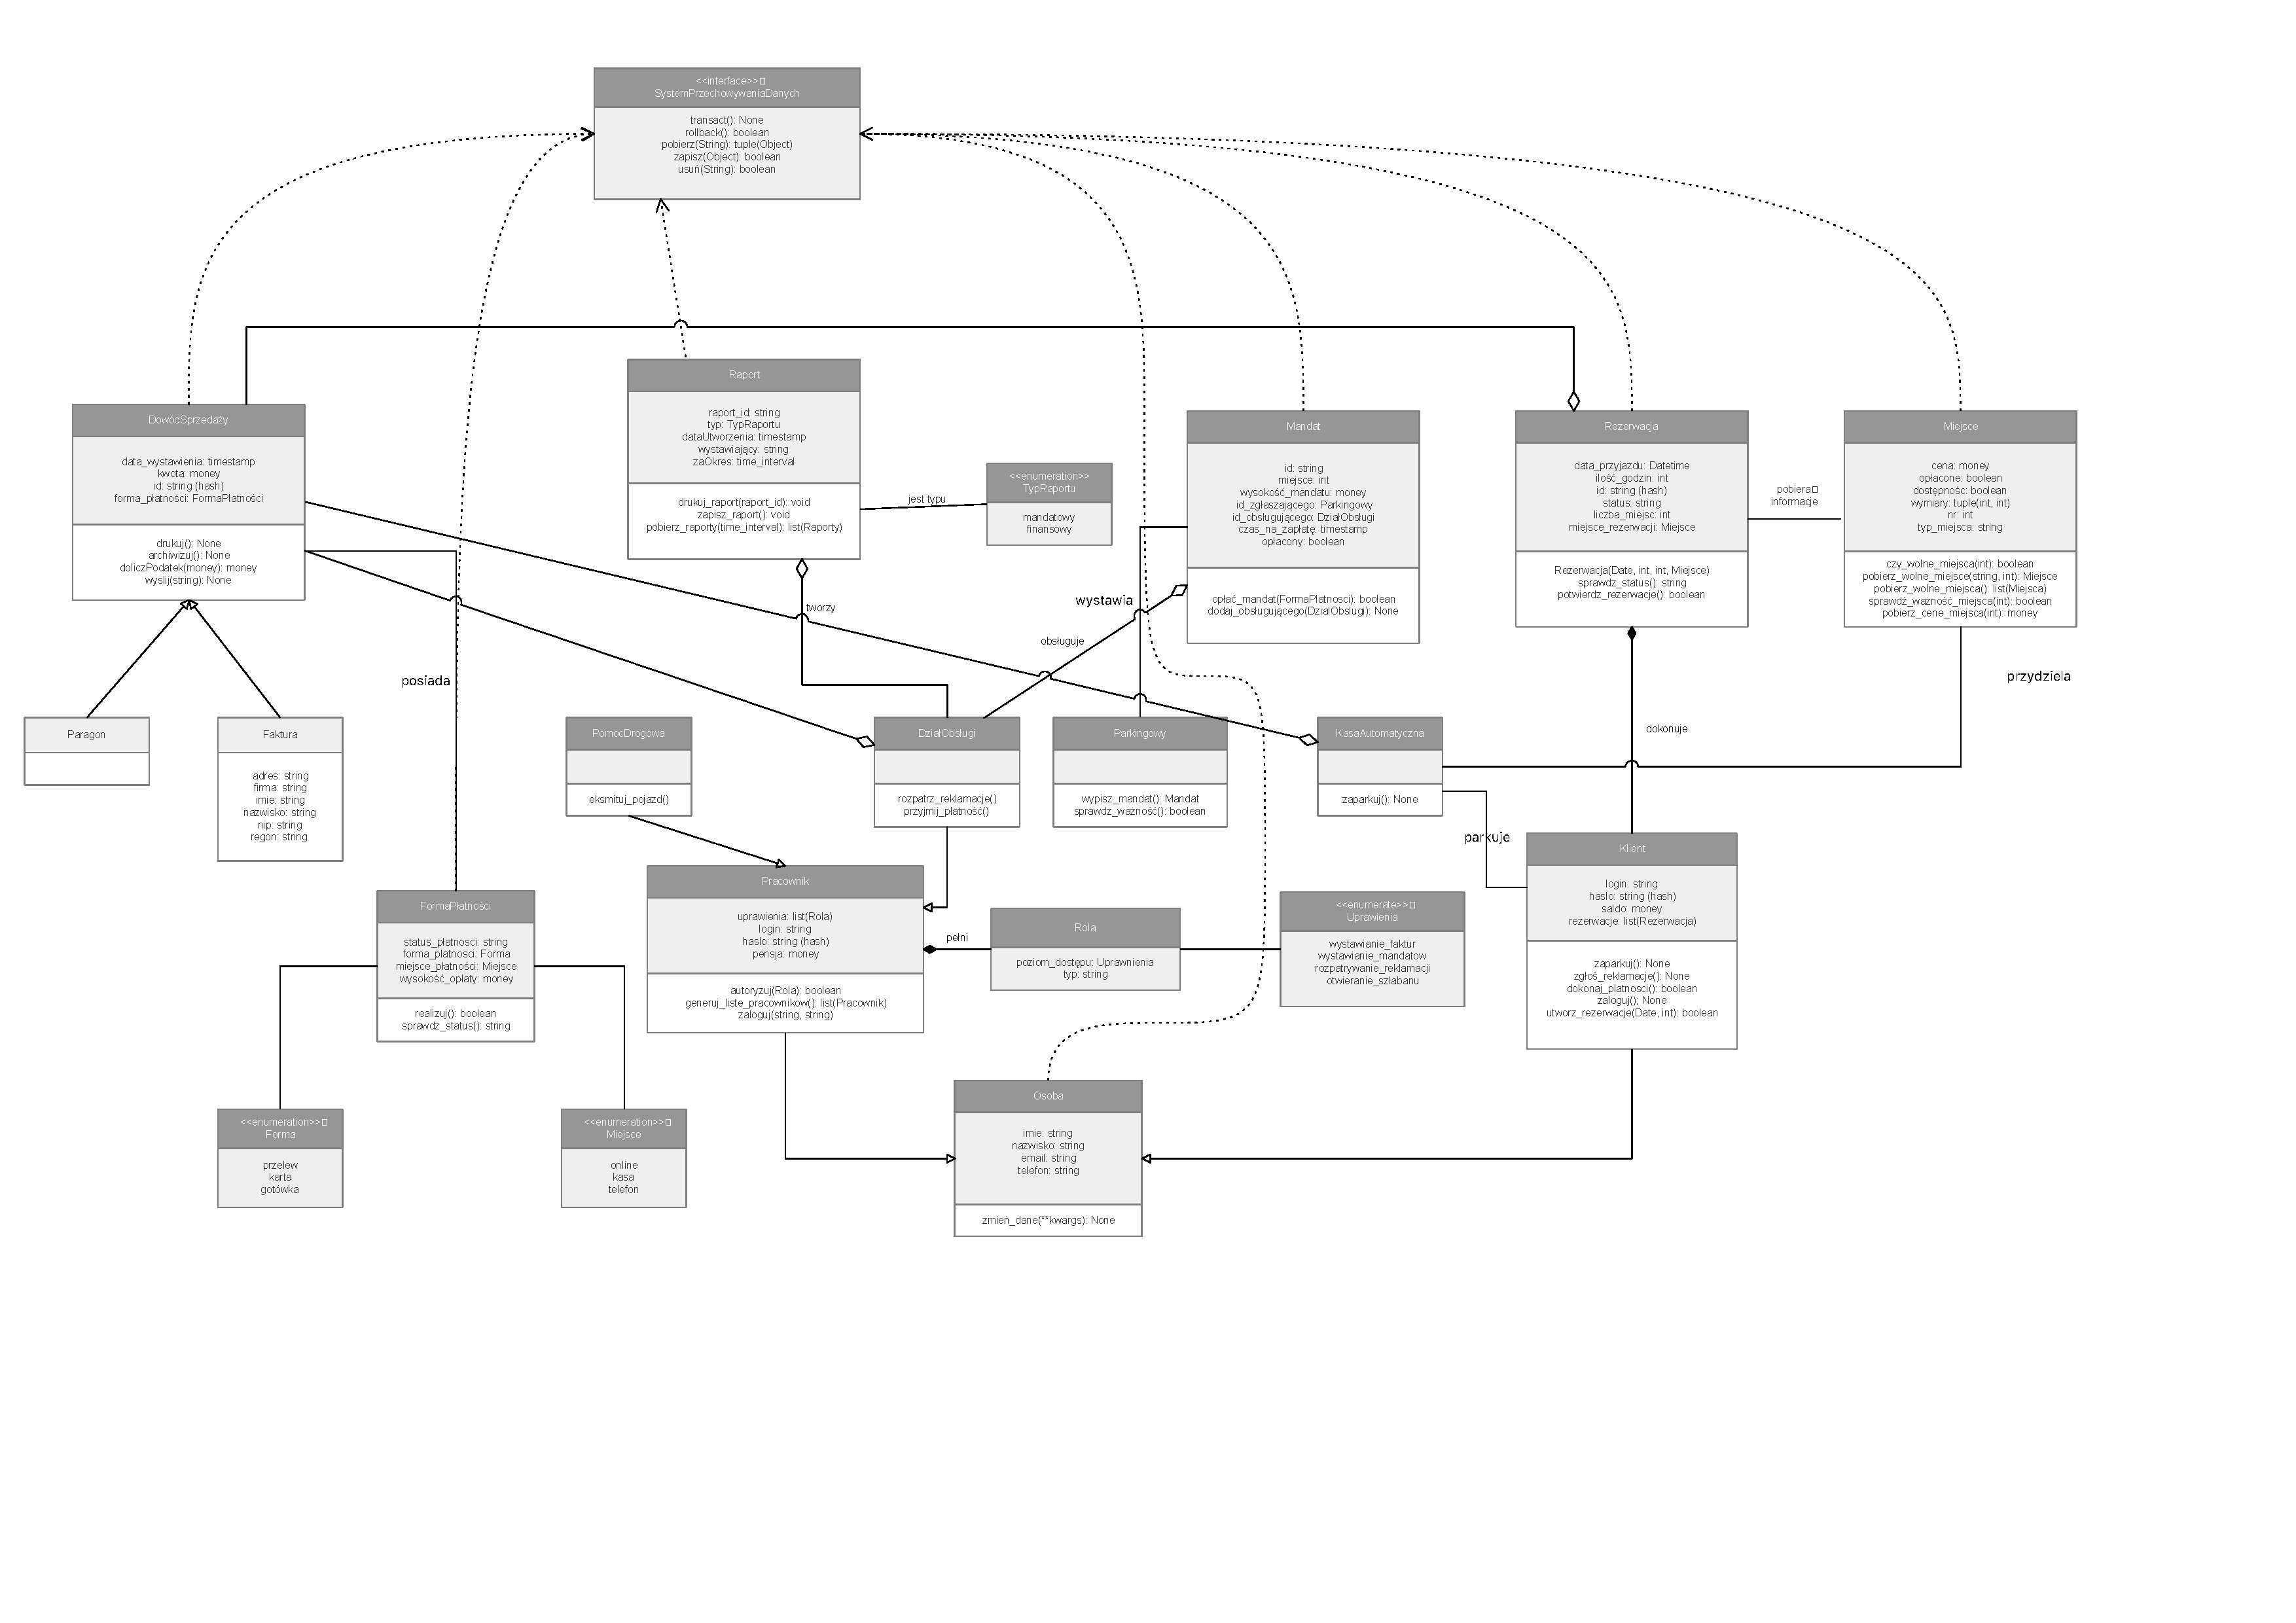
\includepdf[trim=-3cm 0 0 0]{klas/diagram_klas}
\end{figure}
\newpage
\section{Diagramy obiektów}


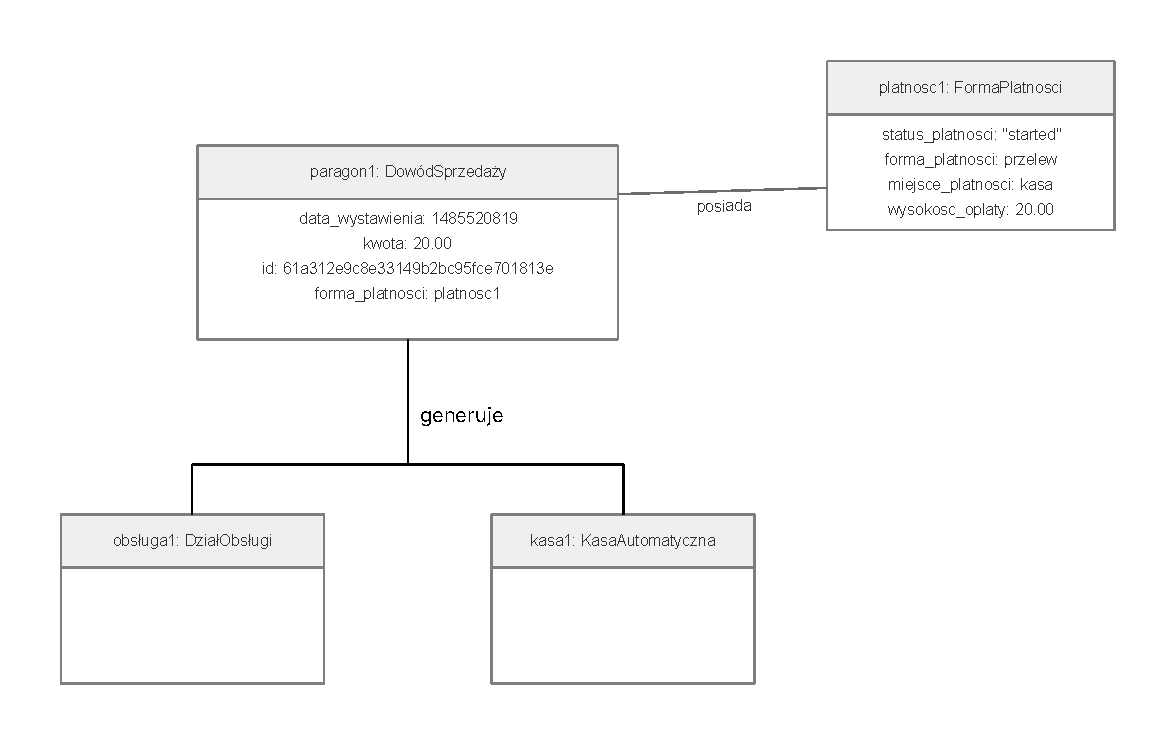
\includepdf[]{obiektow/obiektow-1}
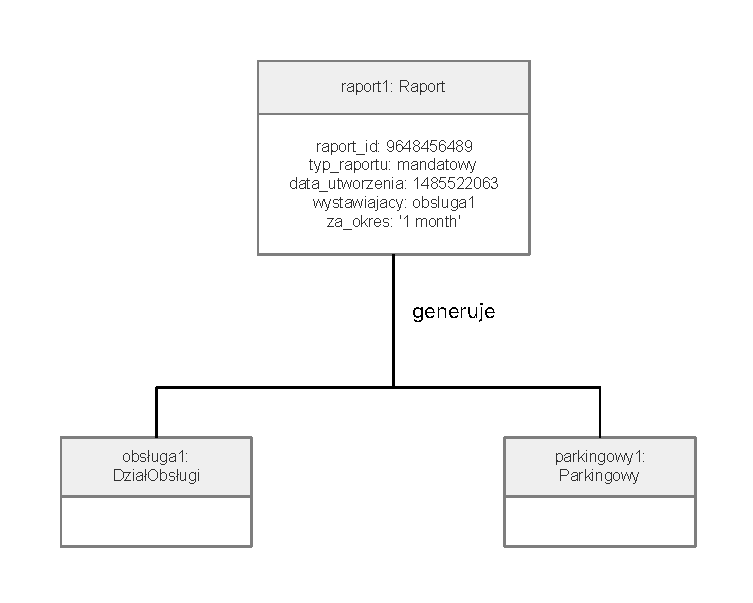
\includepdf[]{obiektow/obiektow-2}
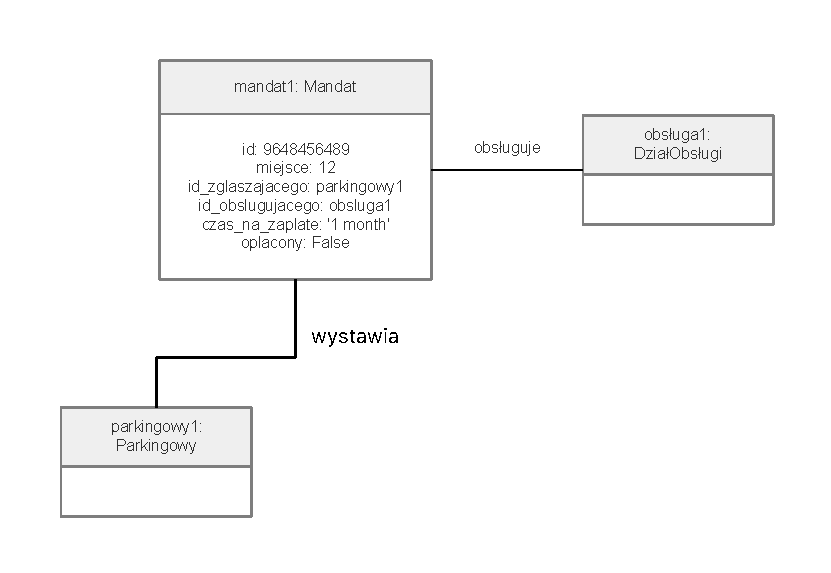
\includepdf[]{obiektow/obiektow-3}
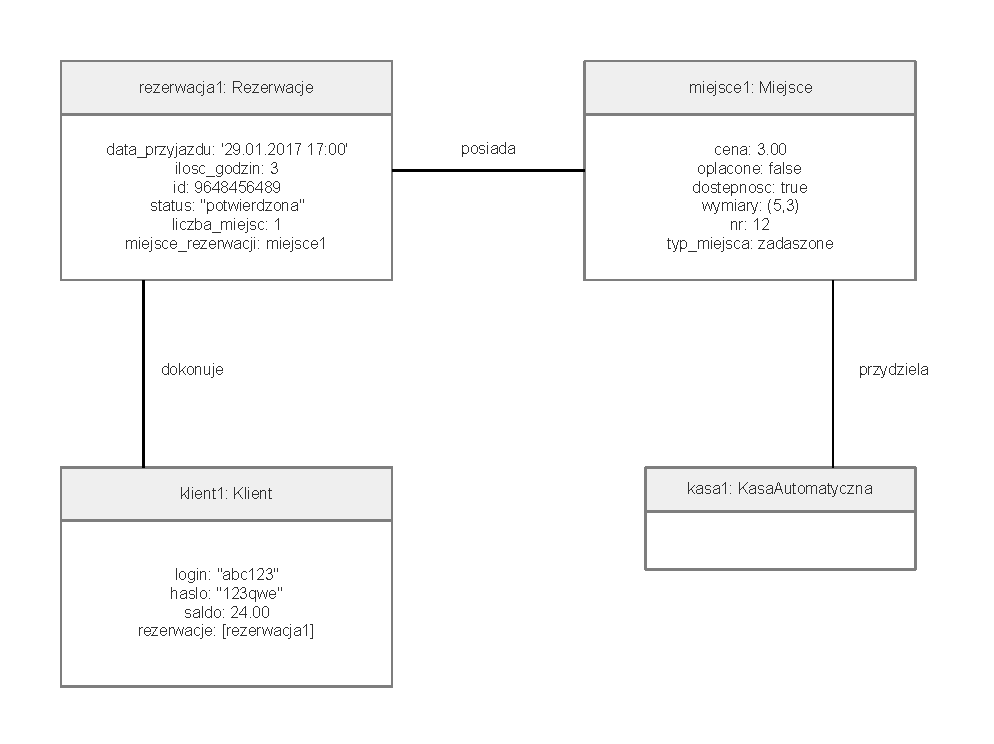
\includepdf[]{obiektow/obiektow-4}
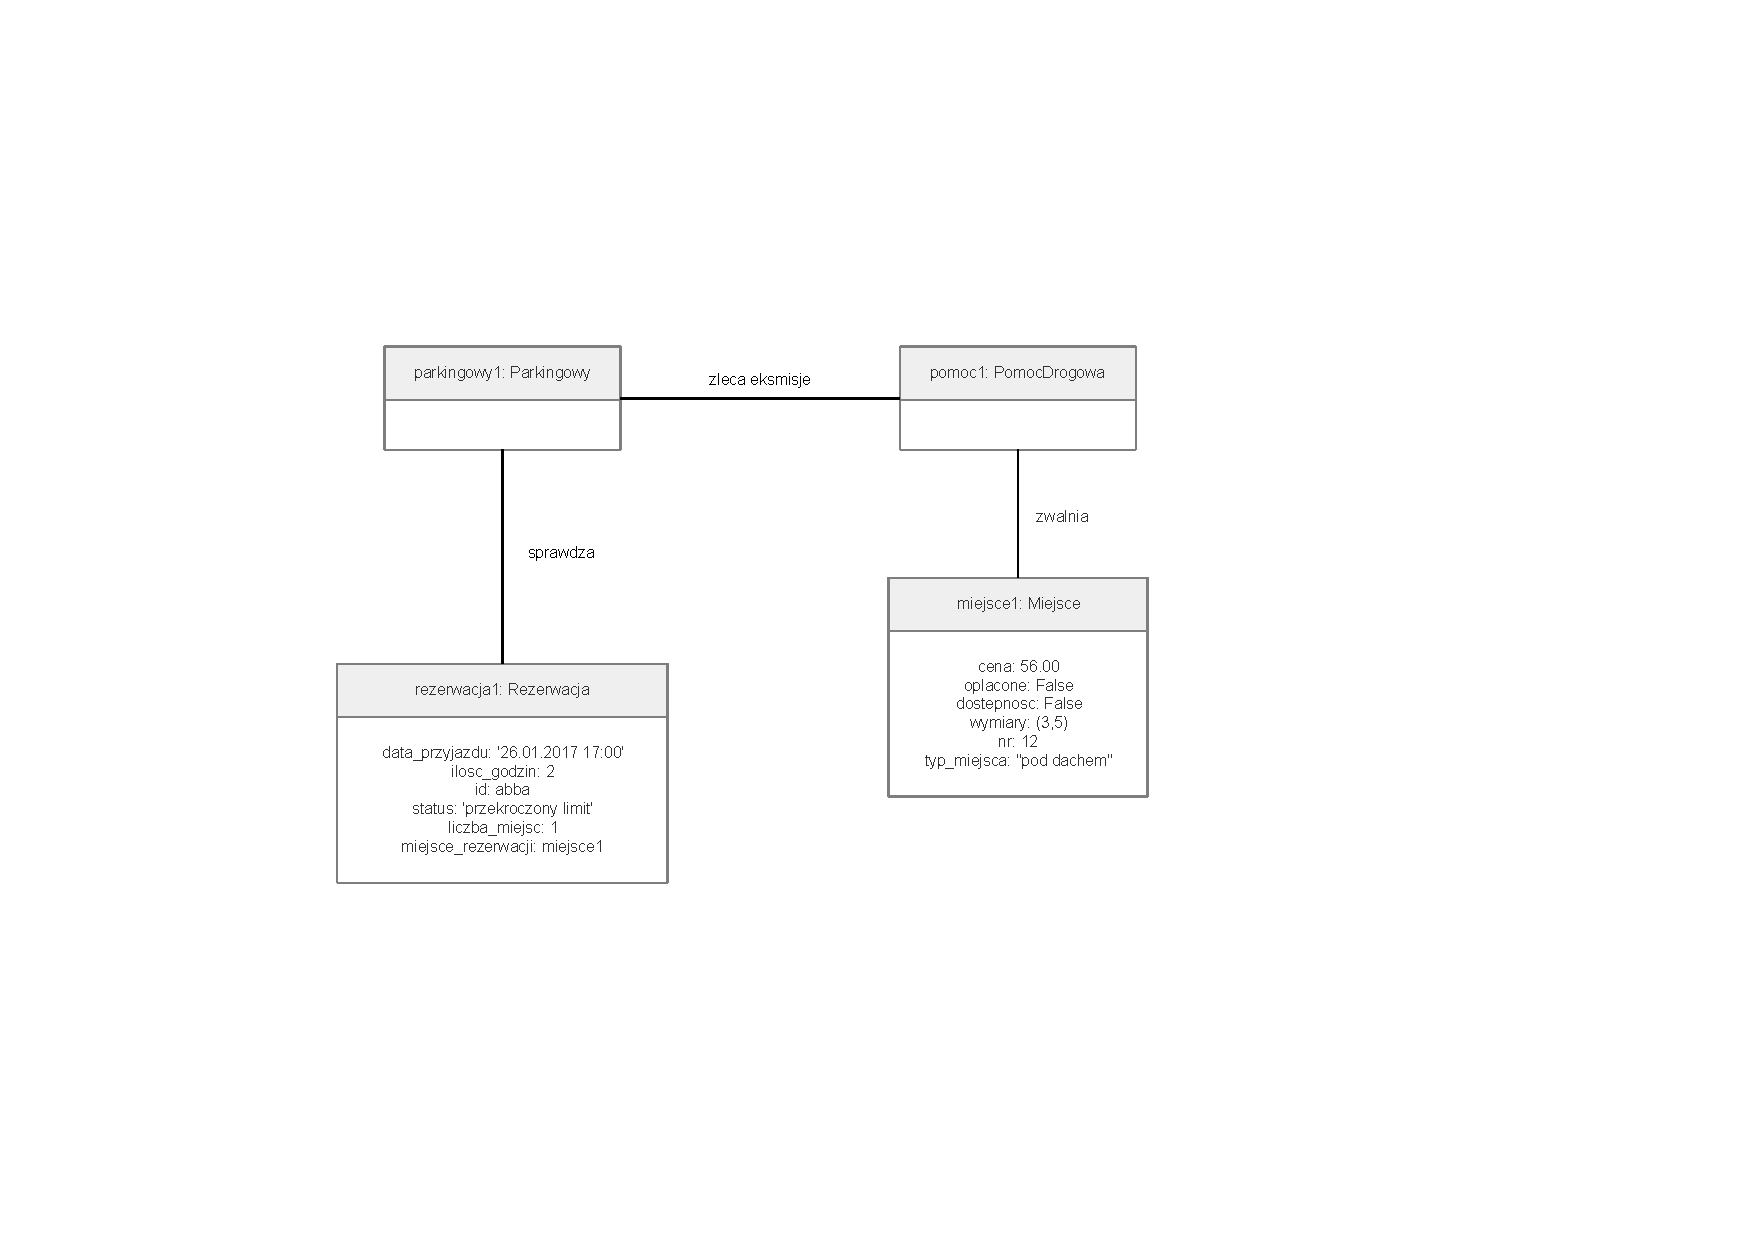
\includepdf[]{obiektow/obiektow-5}
\newpage
\section{Diagramy stanu}

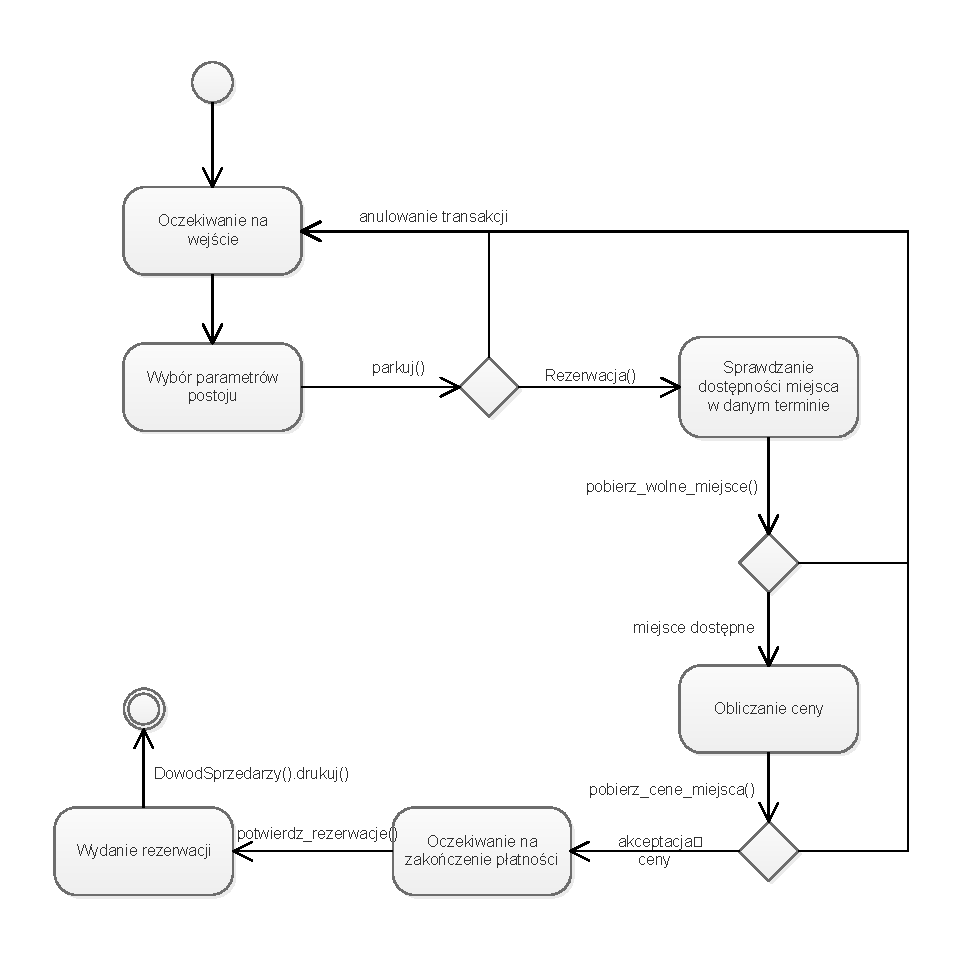
\includepdf[]{stanu/stanu-1}
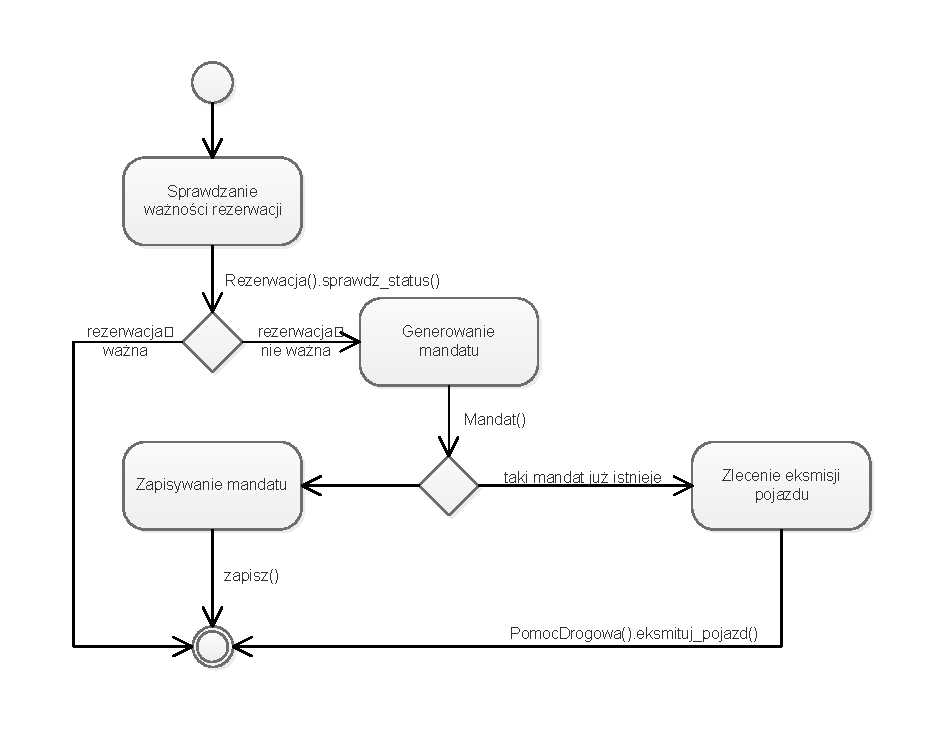
\includepdf[]{stanu/stanu-2}


\end{document}